% !Mode:: "TeX:UTF-8"
\documentclass{apmcmthesis}

\usepackage{url}
\usepackage{booktabs}
\usepackage{graphicx}
\usepackage{amsmath}
\graphicspath{{../outputs/figures/}}

%%%%%%%%%%%% Fill in the team information %%%%%%%%%%%%%%%%%%%%%%%%%%
\tihao{C}
\baominghao{apmcm26XXXXX}

\begin{document}

\pagestyle{frontmatterstyle}

\begin{abstract}
\begin{center}
{\LARGE\bfseries Acoustic Communication and Playback\\[2pt]
Responses of African Penguins at Sea}
\end{center}
\vspace{0.4em}

The African penguin is Critically Endangered and relies on acoustic signals at sea. We
integrate 108 calls, 139 playback experiments and propagation measurements from 4 m to 256 m
to quantify the function and robustness of flat, modulated (mod) and two-voice (tv) calls.

For Problem 1, scalar acoustic measures separate the call types poorly: a random forest reaches
a macro-F1 of 0.385 (permutation $p=0.133$), and flat versus mod is classified at 53.6\%
against a 52.4\% baseline. A structural key using the second voice band and pulse structure
reaches 94.4\%; only peak frequency survives global correction (flat vs.\ mod, $p=0.023$).

For Problem 2, we combine spectrogram, amplitude-spectrum and envelope correlations into a
fidelity index and fit four-parameter logistic curves ($R^2=0.968$--$0.994$). Effective ranges
at thresholds 0.50 and 0.70 are 88.0/42.7 m (flat), 149.7/85.0 m (mod) and 150.4/120.5 m (tv).
The ranking tv $>$ mod $>$ flat holds across six weighting schemes and thresholds from 0.45
to 0.80.

For Problem 3, natural calls raise the group response rate from 12.9\% to 64.7\%
(McNemar $p=7.7\times10^{-20}$); odds ratios relative to control are 14.0, 16.2 and 20.9, and
each doubling of distance multiplies the odds by 0.63 ($p=0.022$). A hurdle model gives median
initiation latencies of 2.0 s, 1.9 s and 2.8 s at 100 m, consistent with the observed 2.05 s.

For Problem 4, the effectiveness index remains highest for tv at 250 m (0.281 versus 0.208 for
flat). A 10\% loss of signal correlation shortens the radius by 4.6\% (tv) to 15.4\% (flat),
and raising the threshold from 0.50 to 0.70 cuts flat calls from 88 m to 43 m but tv only from
150 m to 121 m. Two-voice calls are thus the most robust long-range signal, with conditional
implications for habitat protection and vessel-noise management.

\keywords{African penguin\quad acoustic communication\quad signal degradation\quad playback experiment\quad hurdle model\quad sensitivity analysis}
\end{abstract}

\newpage
{\footnotesize
\tableofcontents
}

\newpage
\pagestyle{mainmatterstyle}
\setcounter{page}{1}

% =====================================================================
\section{Introduction}

\subsection{Background}
The African penguin is listed as Critically Endangered, with an estimated decline of about
8\% per year and a risk of functional extinction in the wild within two decades. The species
breeds, moults and rests on land but forages in coastal waters, where the environment is open,
wave action is strong, and visibility is frequently poor. Under these conditions acoustic
signals are expected to be the main channel for maintaining contact, recognising companions,
and recruiting group members to foraging aggregations.

Human activity at sea introduces ambient noise that may mask these signals. Quantifying how
far each call type remains recognisable, and how strongly penguins respond at that range, is
therefore a prerequisite for evidence-based spatial management.

\subsection{Problem overview}
The problem provides three linked bodies of data: (i) acoustic measurements on 108 calls of
three types (flat, modulated, two-voice); (ii) 139 playback experiments with paired natural-call
and control trials; and (iii) propagation experiments reporting the correlation between signals
recorded at 1 m and at distances from 4 m to 256 m. Four tasks follow: characterise and classify
call types; build a distance-dependent fidelity measure and estimate effective communication
range; model playback responses and response latency; and integrate the results into a
communication-effectiveness index with conservation scenarios.

\subsection{Contributions}
Our contributions are fourfold. First, we show explicitly that the three call types are not
separable by scalar acoustic summaries, but are almost perfectly separated by structural
features (second voice band, pulse structure); this changes how the classification task should
be framed. Second, we build a composite fidelity index, compare three candidate decay models,
and report bootstrapped effective ranges under two recognition criteria plus a full threshold
sweep. Third, we model playback responses with a hurdle structure that treats ``no response''
as a separate process rather than as a long latency, and we report calibrated predictions with
confidence intervals. Fourth, we integrate fidelity and behaviour into an effectiveness index,
test its weight sensitivity, and derive conditional management recommendations.

% =====================================================================
\section{Overall modelling framework}

The four problems form a pipeline rather than four independent essays.
Problem 1 identifies which acoustic properties actually distinguish call types and supplies the
structural dimensions used downstream. Problem 2 turns those dimensions into a
distance-dependent fidelity curve $F_k(d)$ for each call type $k$. Problem 3 supplies the
probability that a group responds, and the latency of that response, as functions of call type,
context, distance and group size. Problem 4 combines the two into an effectiveness index
$E_k(c,d)$ and converts it into radii and expected responder counts.

This chain is reflected in the notation: $k$ indexes call type throughout, $d$ indexes distance,
and the outputs of Problems 2 and 3 enter Problem 4 without refitting.

% =====================================================================
\section{Assumptions}

\begin{enumerate}[label=\textbf{A\arabic*.},leftmargin=*]
\item \textbf{Representativeness.} The 108 calls and 139 experiments represent the False Bay
population in the study period. This is required for any population-level inference and is
limited by the small number of locations (False Bay 105 calls, Seapoint 3).
\item \textbf{Partial independence.} Experiments are independent across \texttt{expID}, but the
call and control trials within an experiment, repeated playback tracks, and same-day trials are
correlated. We absorb this with clustered standard errors and random effects.
\item \textbf{Structural missingness.} Missing second fundamental frequency ($F_{02}$) and
missing pulse rate reflect call anatomy (single-voice calls have no second band; flat calls
have no measurable pulse structure), not random data loss. This is verifiable in the data: all
24 tv calls have $F_{02}$, and all 44 flat calls lack pulse rate.
\item \textbf{1 m reference.} The 1 m recording is treated as the undegraded reference, so all
correlations are relative fidelity rather than absolute perceived quality.
\item \textbf{Monotone degradation.} Fidelity decreases with distance in the large, allowing small
local fluctuations. Without this, a threshold could be crossed several times and the effective
range would not be unique.
\item \textbf{Operational response.} A trial is scored as a response if head-raising, vocalisation
or approach occurs within the observation window. This definition is internally consistent in
the data: \texttt{ResponseYesNo} equals the union of the three behaviours in all 278 rows.
\item \textbf{No response is not non-perception.} A zero means ``not observed within the window'',
not ``not heard''. This is why response probability and latency are modelled separately.
\item \textbf{Separability of effectiveness.} Communication effectiveness can be factorised into
signal fidelity, response probability, and behavioural utility. This is an assumption about the
chain of communication, not a testable property of the data.
\end{enumerate}

% =====================================================================
\section{Notation}

\begin{table}[htbp]
\centering
\caption{Main notation.}
\small
\begin{tabular}{lll}
\toprule
Symbol & Meaning & Type \\
\midrule
$k$ & call type: flat, mod, tv (or control) & index \\
$c$ & context: commuting, searching, after & index \\
$d$ & propagation or playback distance (m) & observed / design \\
$F_{02}, \mathrm{PR}$ & second fundamental frequency; pulse rate & observed \\
$y_i$ & true call type of sample $i$ & observed label \\
$r_{k,m}(d)$ & correlation with the 1 m reference, measure $m$ & observed \\
$F_k(d)$ & composite acoustic fidelity & derived \\
$d_{50,k}, p_k$ & half-decay distance and steepness of the 4PL curve & estimated \\
$\theta$ & recognition threshold & scenario parameter \\
$R_k(\theta)$ & effective communication range (m) & output \\
$N_j$ & number of penguins observed in experiment $j$ & observed \\
$p_j$ & probability that the group responds & estimated \\
$\rho$ & proportion of responsive individuals in a group & assumed \\
$E_k(c,d)$ & communication effectiveness index & output \\
\bottomrule
\end{tabular}
\end{table}

% =====================================================================
\section{Data and preprocessing}

Eleven files were used. Data 01 contains eight acoustic measures on 108 calls (flat 44, mod 40,
tv 24). Data 02 contains 278 trial records from 139 experiments, each with a natural-call and a
control trial. Data 03--11 contain correlation values between the 1 m reference and seven
distances (4, 8, 16, 32, 64, 128, 256 m), for three call types and three representations
(spectrogram, amplitude spectrum, amplitude envelope); each cell contains 190--300 values.

Three preprocessing decisions matter for the results.

\textbf{Response definition.} We verified that \texttt{ResponseYesNo} is exactly the union of
head-raising, vocalisation and approach (0 inconsistencies in 278 rows). Four records coded
\texttt{VocalYesNo}=0 while reporting one or more calls; we defined the vocal event as
``yes or at least one call'', which changes four rows.

\textbf{Missing values.} We did not delete rows with missing $F_{02}$ or pulse rate, because
missingness is structural and deleting it would remove all flat calls from any analysis
including those variables. The scalar classifier therefore uses only the six measures available
for all three types; $F_{02}$ and pulse rate enter the structural key instead.

\textbf{Censoring.} Head-up and approach durations are capped at 60 s, and a large fraction of
trials show no response. Non-response is treated as a separate outcome (hurdle), not as a
latency of zero and not as a missing value.

% =====================================================================
\section{Problem 1: acoustic characteristics and classification}

\subsection{Methods}
Descriptive statistics were computed per call type. Because several measures are skewed and
heteroscedastic, we used Kruskal--Wallis tests for three-group comparisons and pairwise
Mann--Whitney and Kolmogorov--Smirnov tests for post-hoc contrasts, with Holm correction both
within each measure and globally across all 18 pairwise tests. Effect sizes are reported as
$\varepsilon^2$ for Kruskal--Wallis and rank-biserial correlation for Mann--Whitney.

Classifiers were evaluated with five-fold cross-validation \emph{grouped by recording date},
because calls recorded on the same day may come from the same individuals. We report a global
majority baseline, a logistic regression and a random forest on the six common scalar measures,
a label-permutation test, and a structural diagnostic key. The key is a deterministic rule
based on call anatomy: presence of $F_{02}$ indicates tv; otherwise presence of pulse rate
indicates mod; otherwise flat. A model using missingness indicators is reported only as a
\emph{leakage upper bound}, because those indicators are deterministic functions of the label.

\subsection{Results}
Peak frequency, first fundamental frequency and median spectral frequency differ among call
types (Table~\ref{tab:kw}). After global multiplicity correction, however, only the flat versus
mod contrast in peak frequency remains significant ($p=0.023$, rank-biserial $=0.41$).
Duration, the 25th percentile and the 75th percentile do not differ.

\begin{table}[htbp]
\centering
\caption{Kruskal--Wallis tests and the only pairwise contrast surviving global Holm correction.}
\label{tab:kw}
\small
\begin{tabular}{lcccl}
\toprule
Measure & $H$ & $p$ & $\varepsilon^2$ & Significant pairwise contrast \\
\midrule
Duration & 2.52 & 0.283 & 0.005 & --- \\
$F_{01}$ & 9.14 & 0.010 & 0.068 & --- (flat vs.\ tv, global $p=0.124$) \\
Peak frequency & 12.28 & 0.002 & 0.098 & flat vs.\ mod, global $p=0.023$ \\
$Q_{25}$ & 2.16 & 0.340 & 0.001 & --- \\
$Q_{50}$ & 6.43 & 0.040 & 0.042 & --- (flat vs.\ mod, global $p=0.668$) \\
$Q_{75}$ & 0.52 & 0.771 & 0.000 & --- \\
\bottomrule
\end{tabular}
\end{table}

\begin{figure}[htbp]
\centering
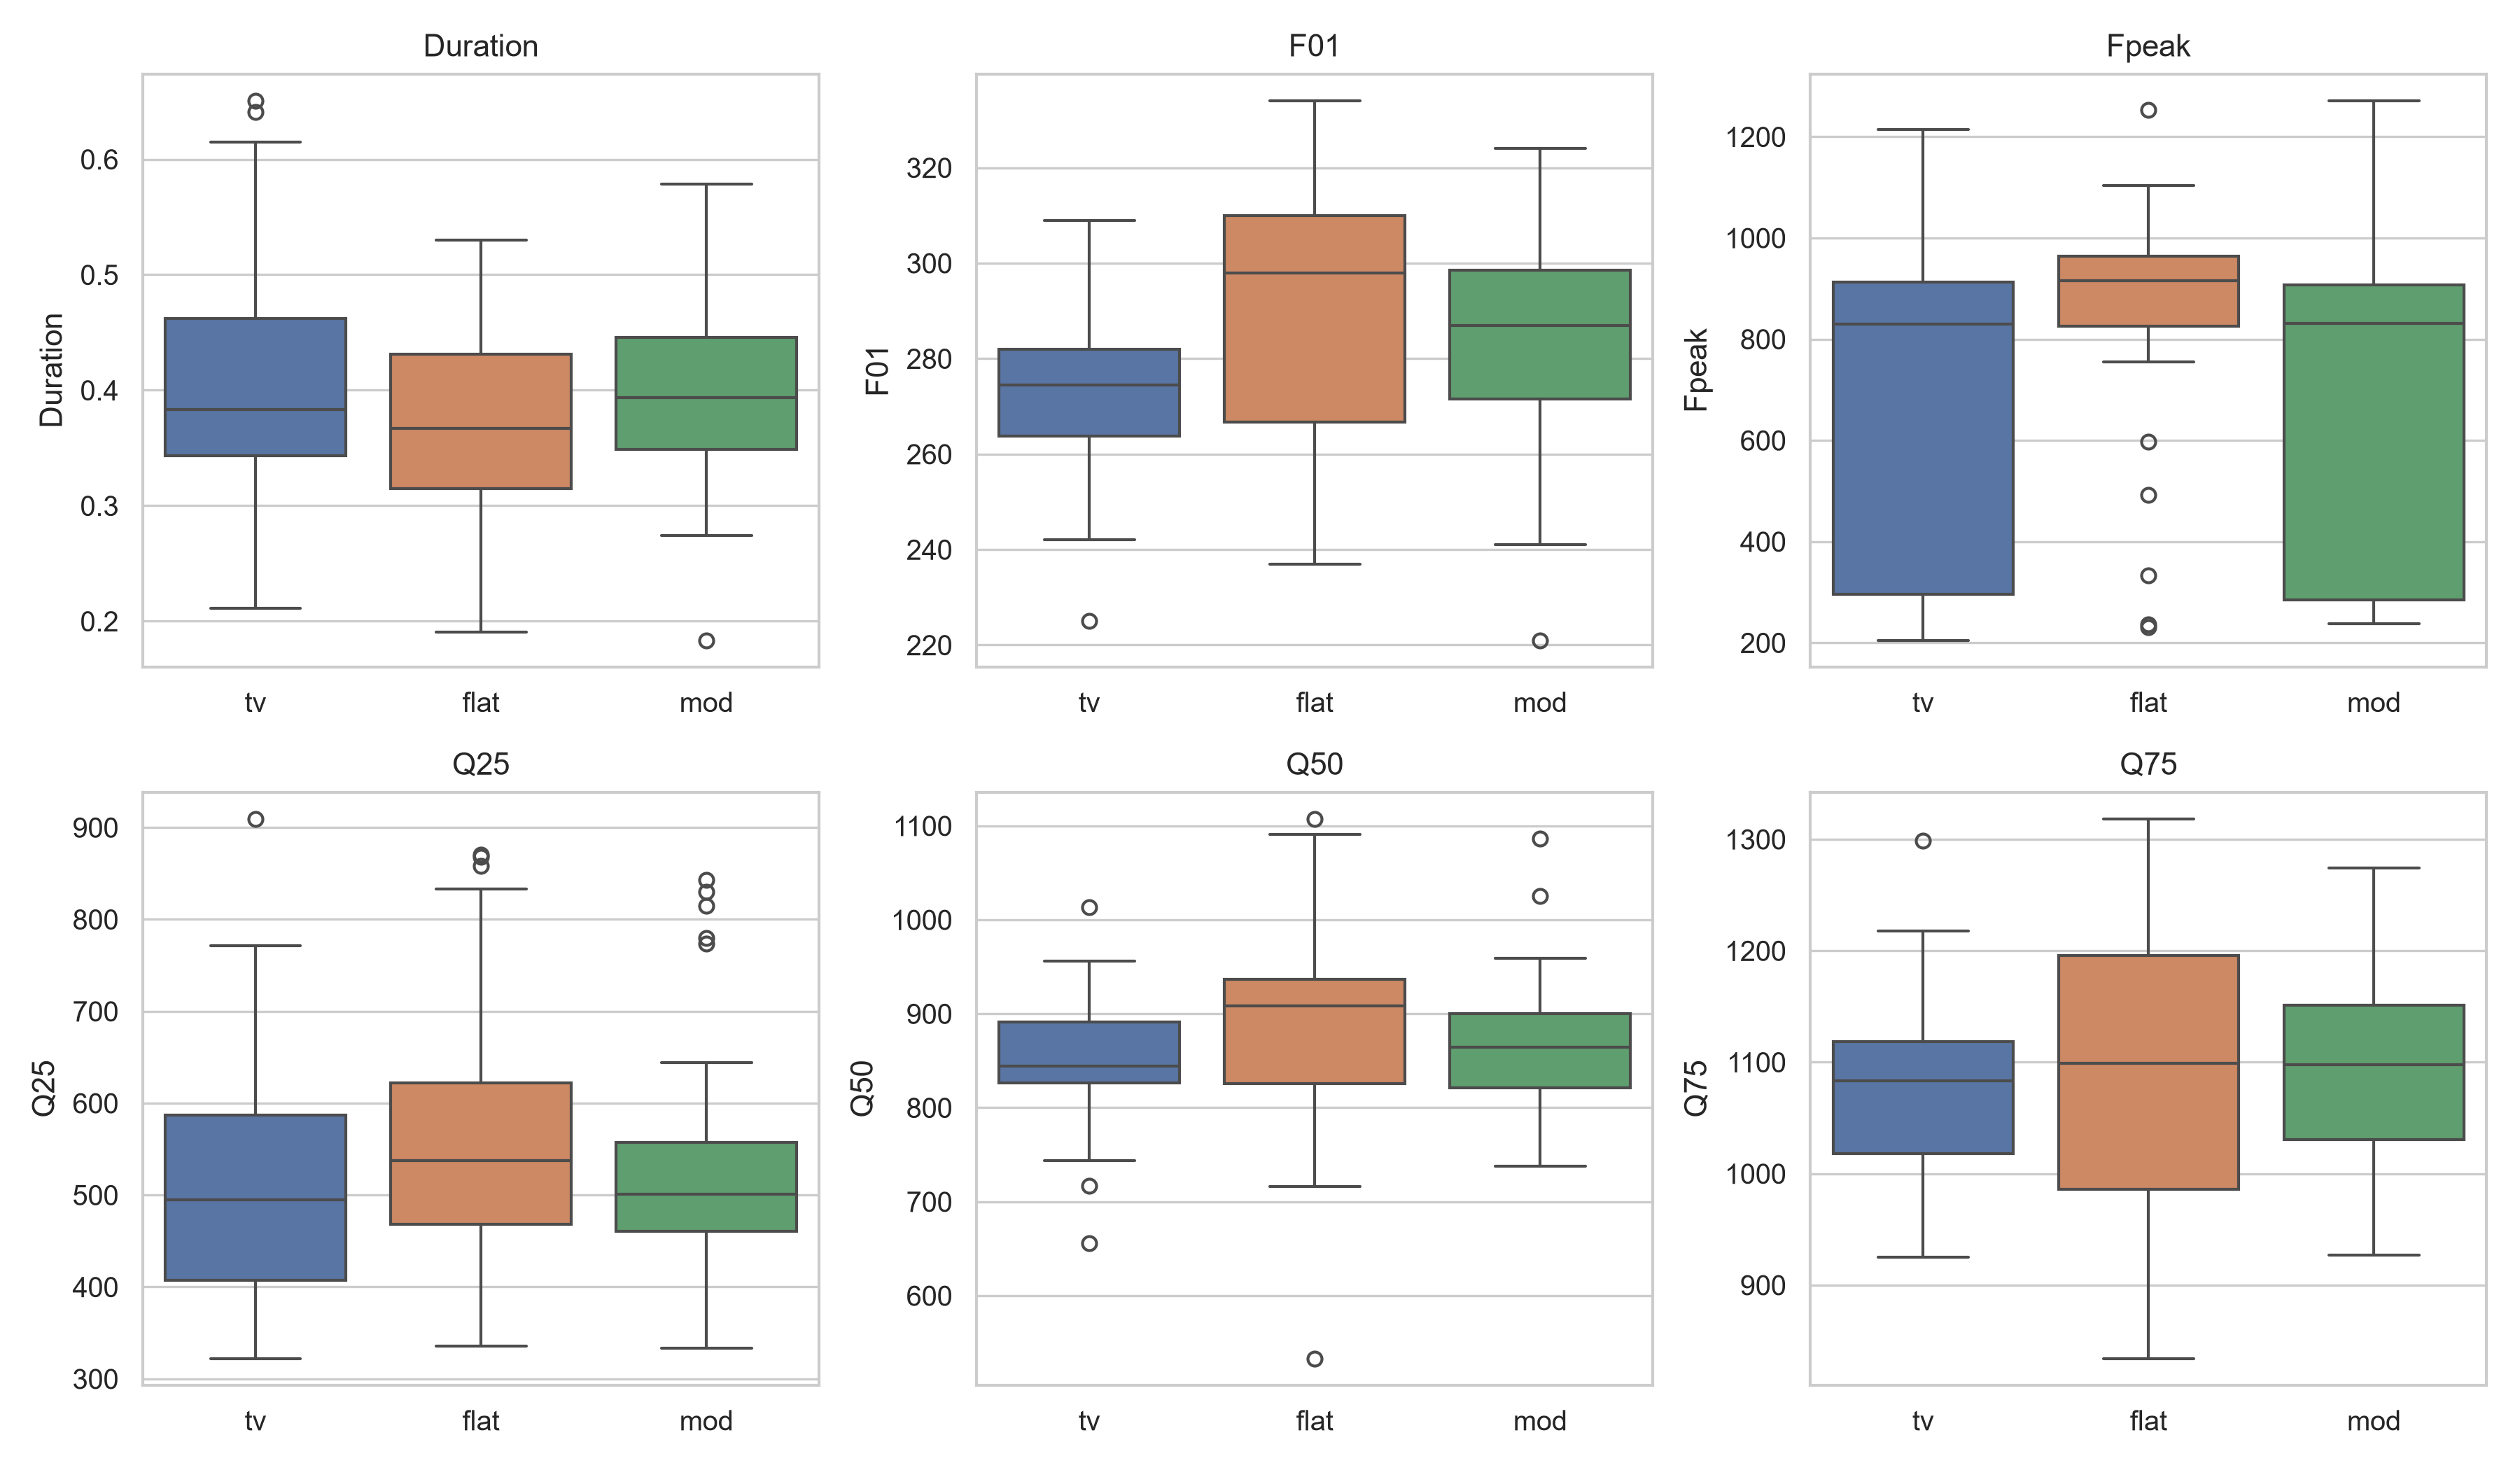
\includegraphics[width=0.95\textwidth]{q1_feature_boxplot.png}
\caption{Distributions of the eight acoustic measures by call type. $F_{02}$ is present only
for tv calls and pulse rate is absent for flat calls, so those panels also display the
structural definition of the call types.}
\label{fig:q1box}
\end{figure}

Classification results are shown in Table~\ref{tab:clf} and Figure~\ref{fig:q1cm}. The scalar
classifier performs poorly. The random forest reaches 43.5\% accuracy and a macro-F1 of 0.385,
against 40.7\% and 0.193 for always predicting flat; the permutation test gives $p=0.133$, so
the improvement is not distinguishable from chance at the 5\% level. Recall for tv is only
0.125. Restricting to single-voice calls, where flat and mod are nearly balanced (44 vs.\ 40),
the random forest reaches 53.6\% against a 52.4\% majority baseline. The structural key, by
contrast, classifies 94.4\% correctly (macro-F1 0.952), misclassifying only six mod calls that
lack measurable pulse rate.

\begin{table}[htbp]
\centering
\caption{Classification performance under cross-validation grouped by recording date.}
\label{tab:clf}
\small
\resizebox{\textwidth}{!}{%
\begin{tabular}{lcccc}
\toprule
Model & Accuracy & Balanced accuracy & Macro-F1 & Recall (flat/mod/tv) \\
\midrule
Global majority & 0.407 & 0.333 & 0.193 & 1.00 / 0.00 / 0.00 \\
Logistic regression, 6 measures & 0.407 & 0.358 & 0.345 & 0.59 / 0.40 / 0.08 \\
Random forest, 6 measures & 0.435 & 0.391 & 0.385 & 0.52 / 0.53 / 0.13 \\
\emph{Leakage upper bound} (with missingness indicators) & 0.648 & 0.603 & 0.603 & 0.75 / 0.73 / 0.33 \\
Structural key (F$_{02}$ / pulse rate) & 0.944 & 0.950 & 0.952 & 1.00 / 0.85 / 1.00 \\
\bottomrule
\end{tabular}}
\end{table}

\begin{figure}[htbp]
\centering
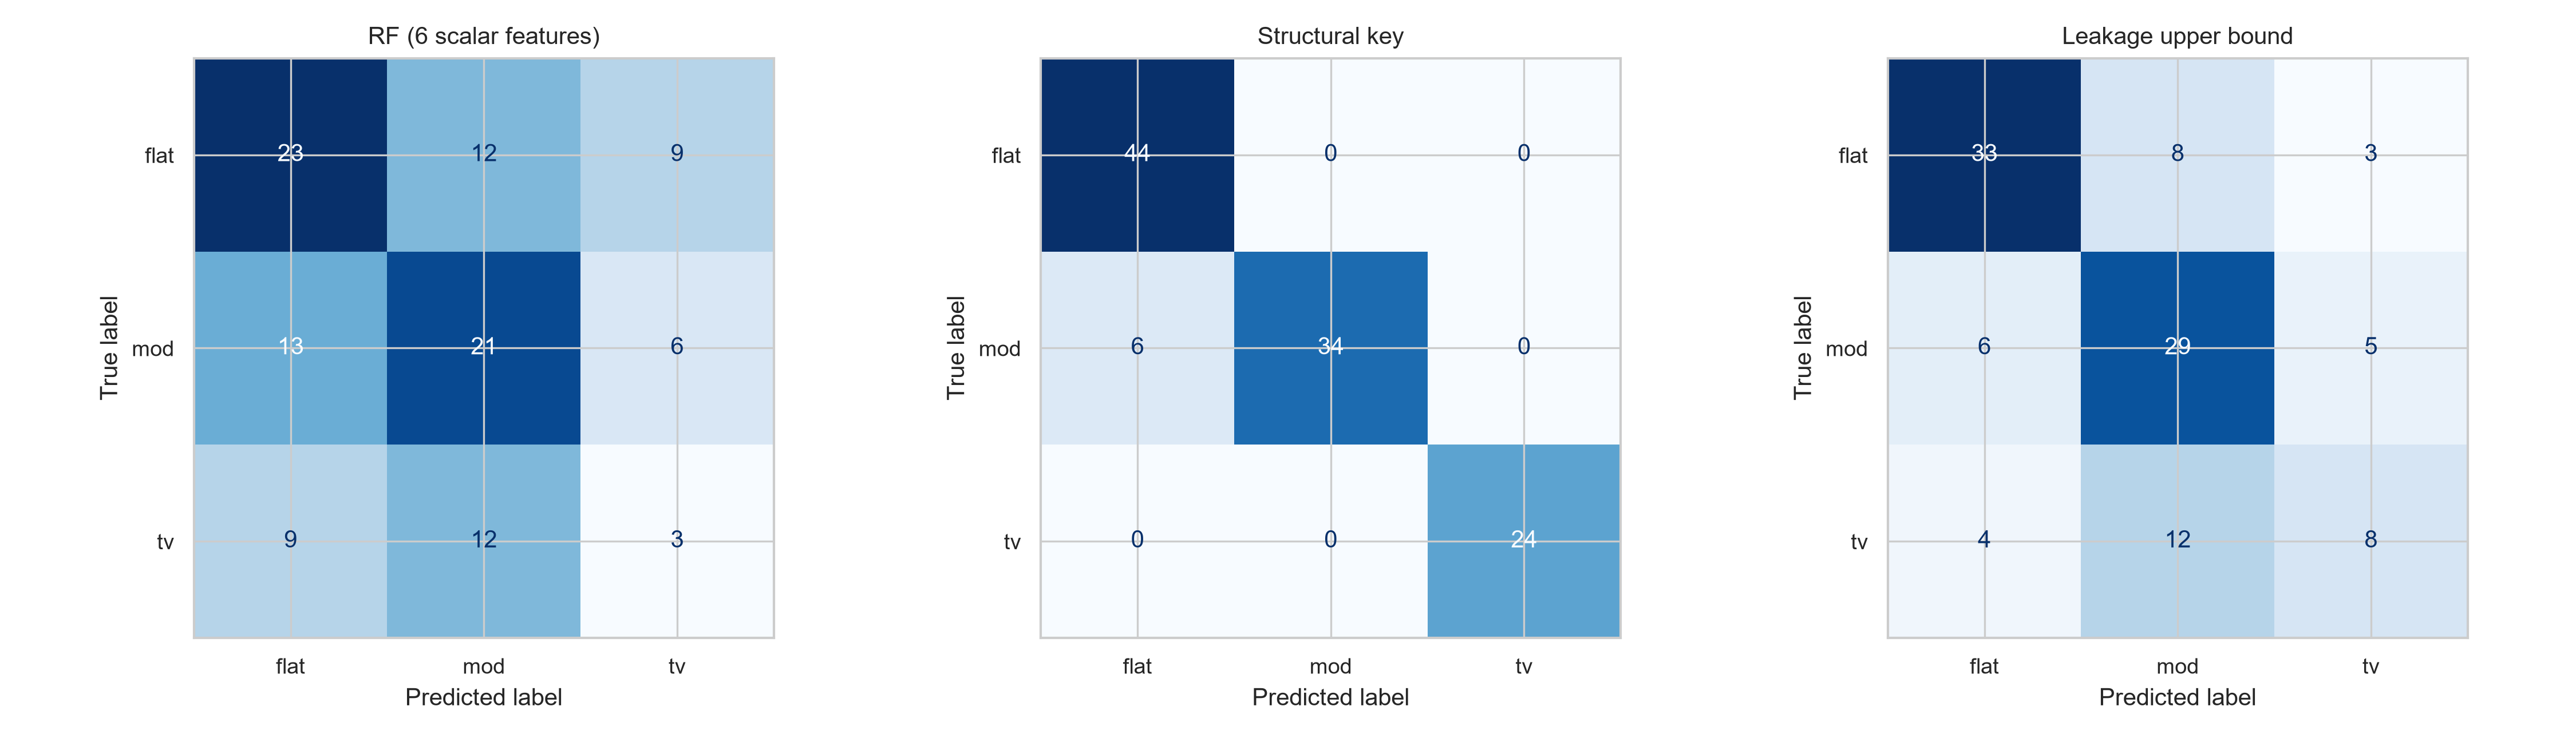
\includegraphics[width=0.95\textwidth]{q1_confusion_matrices.png}
\caption{Confusion matrices for the scalar random forest, the structural key, and the leakage
upper bound. The scalar model almost never identifies tv calls.}
\label{fig:q1cm}
\end{figure}

\subsection{Interpretation and key measures}
The three call types are not distinguished by how long or how high-pitched they are, but by
whether a second voice band is present and whether pulse structure is measurable. This is a
substantive result, not a failure of the classifier: it says that the information distinguishing
the call types is carried by spectral and temporal structure, which scalar summaries discard.
It also explains why we adopt three structural fidelity dimensions in Problem 2---spectrogram
(frequency modulation over time), amplitude spectrum (frequency content) and envelope (temporal
amplitude modulation)---rather than a single acoustic index.

% =====================================================================
\section{Problem 2: propagation degradation and effective range}

\subsection{Composite fidelity index}
For each call type and measure $m\in\{\text{spectrogram},\text{amplitude spectrum},\text{envelope}\}$,
the data provide correlation $r_{k,m}(d)$ with the 1 m reference. We combine the three
measures into a weighted index
\begin{equation}
F_k(d)=\sum_{m} w_m\,r_{k,m}(d),\qquad \sum_m w_m=1,
\end{equation}
with weights obtained by principal-component analysis of the pooled, complete observations
(spectrogram 0.356, amplitude spectrum 0.346, envelope 0.298). The weights are nearly equal.
Because the mean envelope correlation never exceeds about 0.75, the composite at 4 m is
0.76--0.84 rather than 1.0; thresholds must therefore be read as \emph{relative} to the best
available recording, not as absolute recognition probabilities.
This also matters because the spectrogram and amplitude-spectrum correlations are almost the same
variable for mod and tv ($r=0.91$--$0.99$ at most distances), whereas for flat they diverge at
intermediate distances ($r=0.56$--$0.62$ at 32--64 m). The composite therefore represents
spectral structure twice for mod and tv. We retain it as the baseline but test five alternative
weighting schemes (equal, entropy, and each single measure) in Section~\ref{sec:q2sens}.

\subsection{Degradation model}
We fitted three candidate models to the distance means: exponential, log-linear, and a
four-parameter logistic (4PL)
\begin{equation}
F(d)=F_{\min}+\frac{F_{\max}-F_{\min}}{1+(d/d_{50})^{p}}.
\end{equation}
The 4PL provided the best fit for all three call types (Table~\ref{tab:q2models}). It captures
the observed shape: a plateau to about 64 m, a steep decline between 64 and 128 m, and an
asymptote at long range. $R^2$ ranges from 0.968 (tv) to 0.994 (flat); AIC is lowest for the 4PL
in every case. Fitting to the seven distance means (rather than to all individual values) is a
deliberate choice: it makes the fitted curve describe the population mean, and it avoids
letting the unequal number of valid observations per distance drive the shape. The cost is that
$R^2$ describes only seven points and should not be read as a conventional goodness-of-fit on
19{,}000 observations.

\begin{table}[htbp]
\centering
\caption{Model comparison for the composite fidelity curve.}
\label{tab:q2models}
\small
\begin{tabular}{llccc}
\toprule
Call type & Model & $R^2$ & RMSE & AIC \\
\midrule
flat & Exponential & 0.987 & 0.027 & $-44.7$ \\
flat & Log-linear & 0.968 & 0.042 & $-38.2$ \\
flat & 4PL & \textbf{0.994} & \textbf{0.018} & $\mathbf{-48.4}$ \\
mod & Exponential & 0.932 & 0.052 & $-35.4$ \\
mod & Log-linear & 0.970 & 0.034 & $-41.2$ \\
mod & 4PL & \textbf{0.978} & \textbf{0.029} & $\mathbf{-41.4}$ \\
tv & Exponential & 0.812 & 0.071 & $-30.9$ \\
tv & Log-linear & 0.876 & 0.058 & $-33.8$ \\
tv & 4PL & \textbf{0.968} & \textbf{0.029} & $\mathbf{-41.3}$ \\
\bottomrule
\end{tabular}
\end{table}

\subsection{Effective communication range}
For a threshold $\theta$ we solve $F_k(d)=\theta$ numerically on $[1,1000]$ m. Uncertainty is
obtained by bootstrapping the individual correlation values 500 times, refitting the curve and
re-solving. Table~\ref{tab:q2range} reports the two criteria emphasised in the problem
(potential recognition 0.50; reliable recognition 0.70) plus an intermediate level (0.60).
At 0.50 the ranges are 88 m, 150 m and 150 m for flat, mod and tv; at 0.70 they fall to 43 m,
85 m and 121 m. The ordering tv $>$ mod $>$ flat holds at every threshold.

\begin{table}[htbp]
\centering
\caption{Effective communication range (m) with 95\% bootstrap intervals.}
\label{tab:q2range}
\small
\begin{tabular}{lccc}
\toprule
Call type & $\theta=0.50$ (potential) & $\theta=0.60$ & $\theta=0.70$ (reliable) \\
\midrule
flat & 88.0 (85.8--90.3) & 64.4 (62.5--66.7) & 42.7 (40.6--45.0) \\
mod & 149.7 (143.7--153.2) & 118.0 (114.5--121.9) & 85.0 (82.3--91.2) \\
tv & 150.4 (149.1--151.7) & 137.7 (136.7--138.8) & 120.5 (119.5--121.5) \\
\bottomrule
\end{tabular}
\end{table}

\begin{figure}[htbp]
\centering
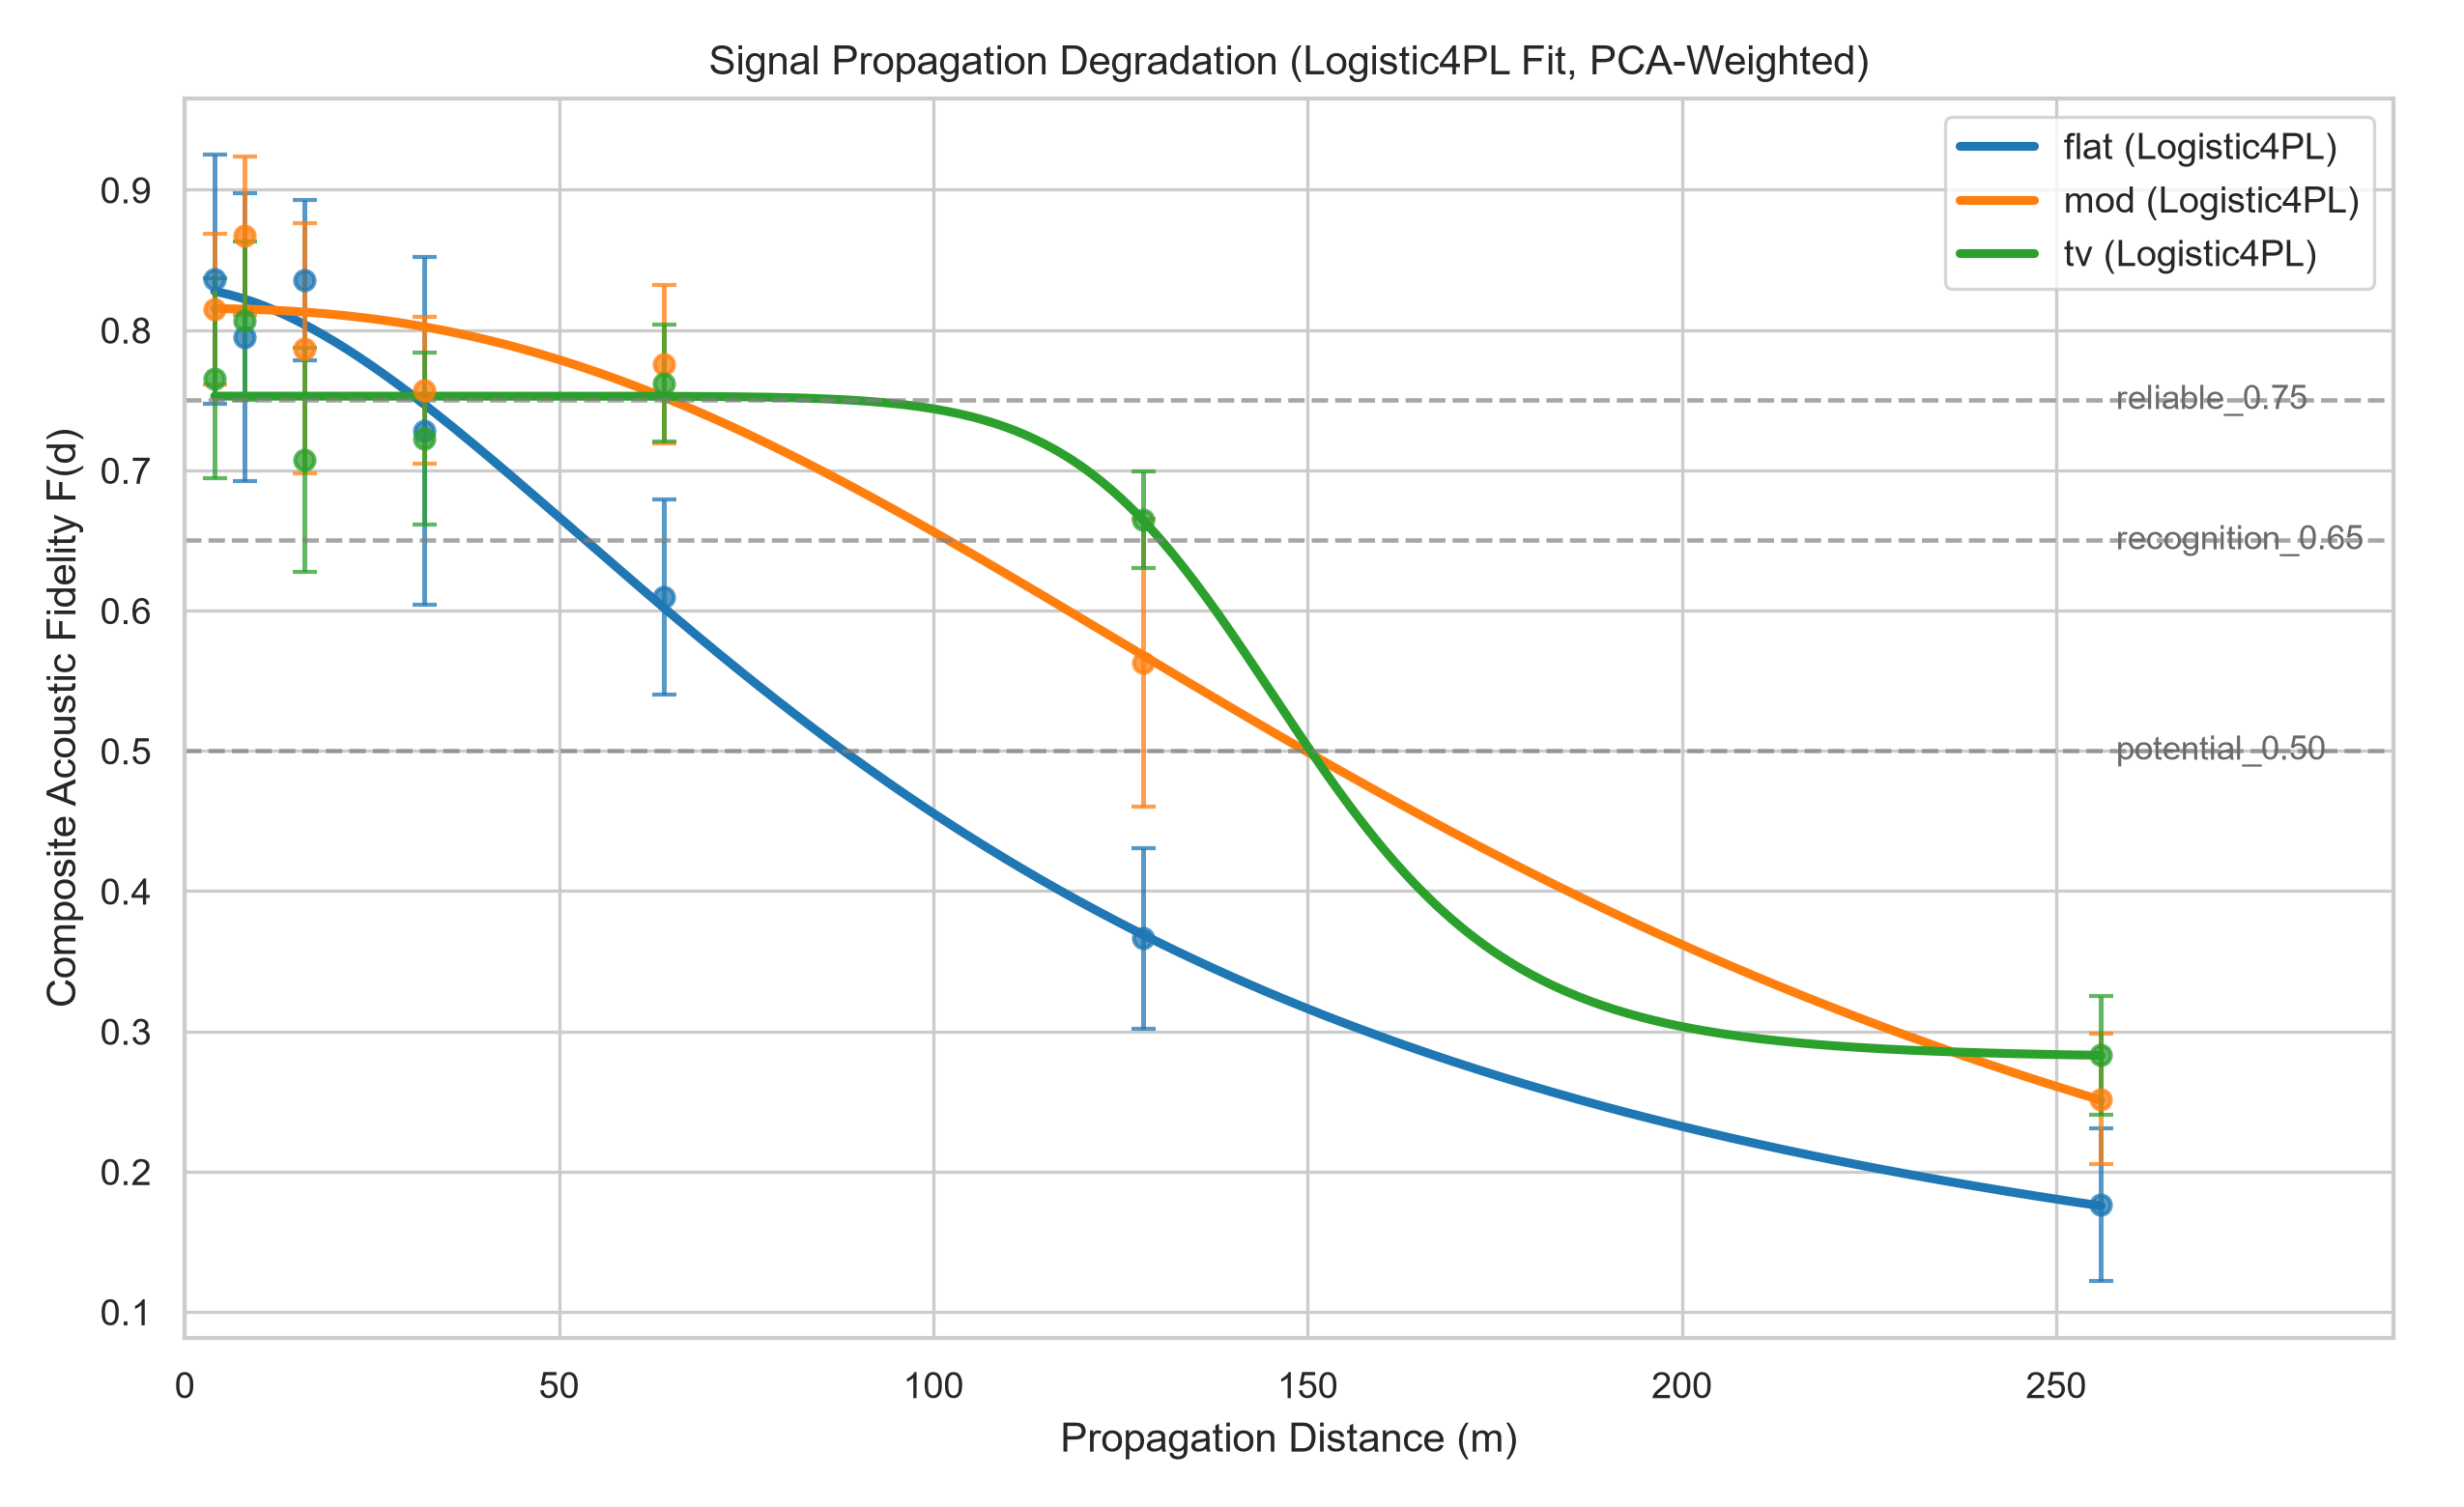
\includegraphics[width=0.95\textwidth]{q2_degradation_curves.png}
\caption{Composite fidelity versus distance with the fitted 4PL curves. Horizontal dashed lines
mark the three recognition thresholds.}
\label{fig:q2curves}
\end{figure}

\subsection{Sensitivity}
\label{sec:q2sens}
Two sensitivities are reported. First, thresholds from 0.45 to 0.80 change the radii smoothly
and preserve the ranking; Table~\ref{tab:q2range} reports the 0.50, 0.60 and 0.70 cases.
Second, weighting scheme matters
more than threshold choice for flat: at $\theta=0.50$ the flat radius is 38.0 m with
envelope-only weights but 110.6 m with amplitude-spectrum-only weights. The corresponding
ranges are 76.9--168.8 m for mod and 105.9--169.7 m for tv. The ranking is nevertheless
preserved in all six schemes. We therefore report the composite result as the baseline and
treat the single-measure values as its plausible bounds.

\begin{figure}[htbp]
\centering
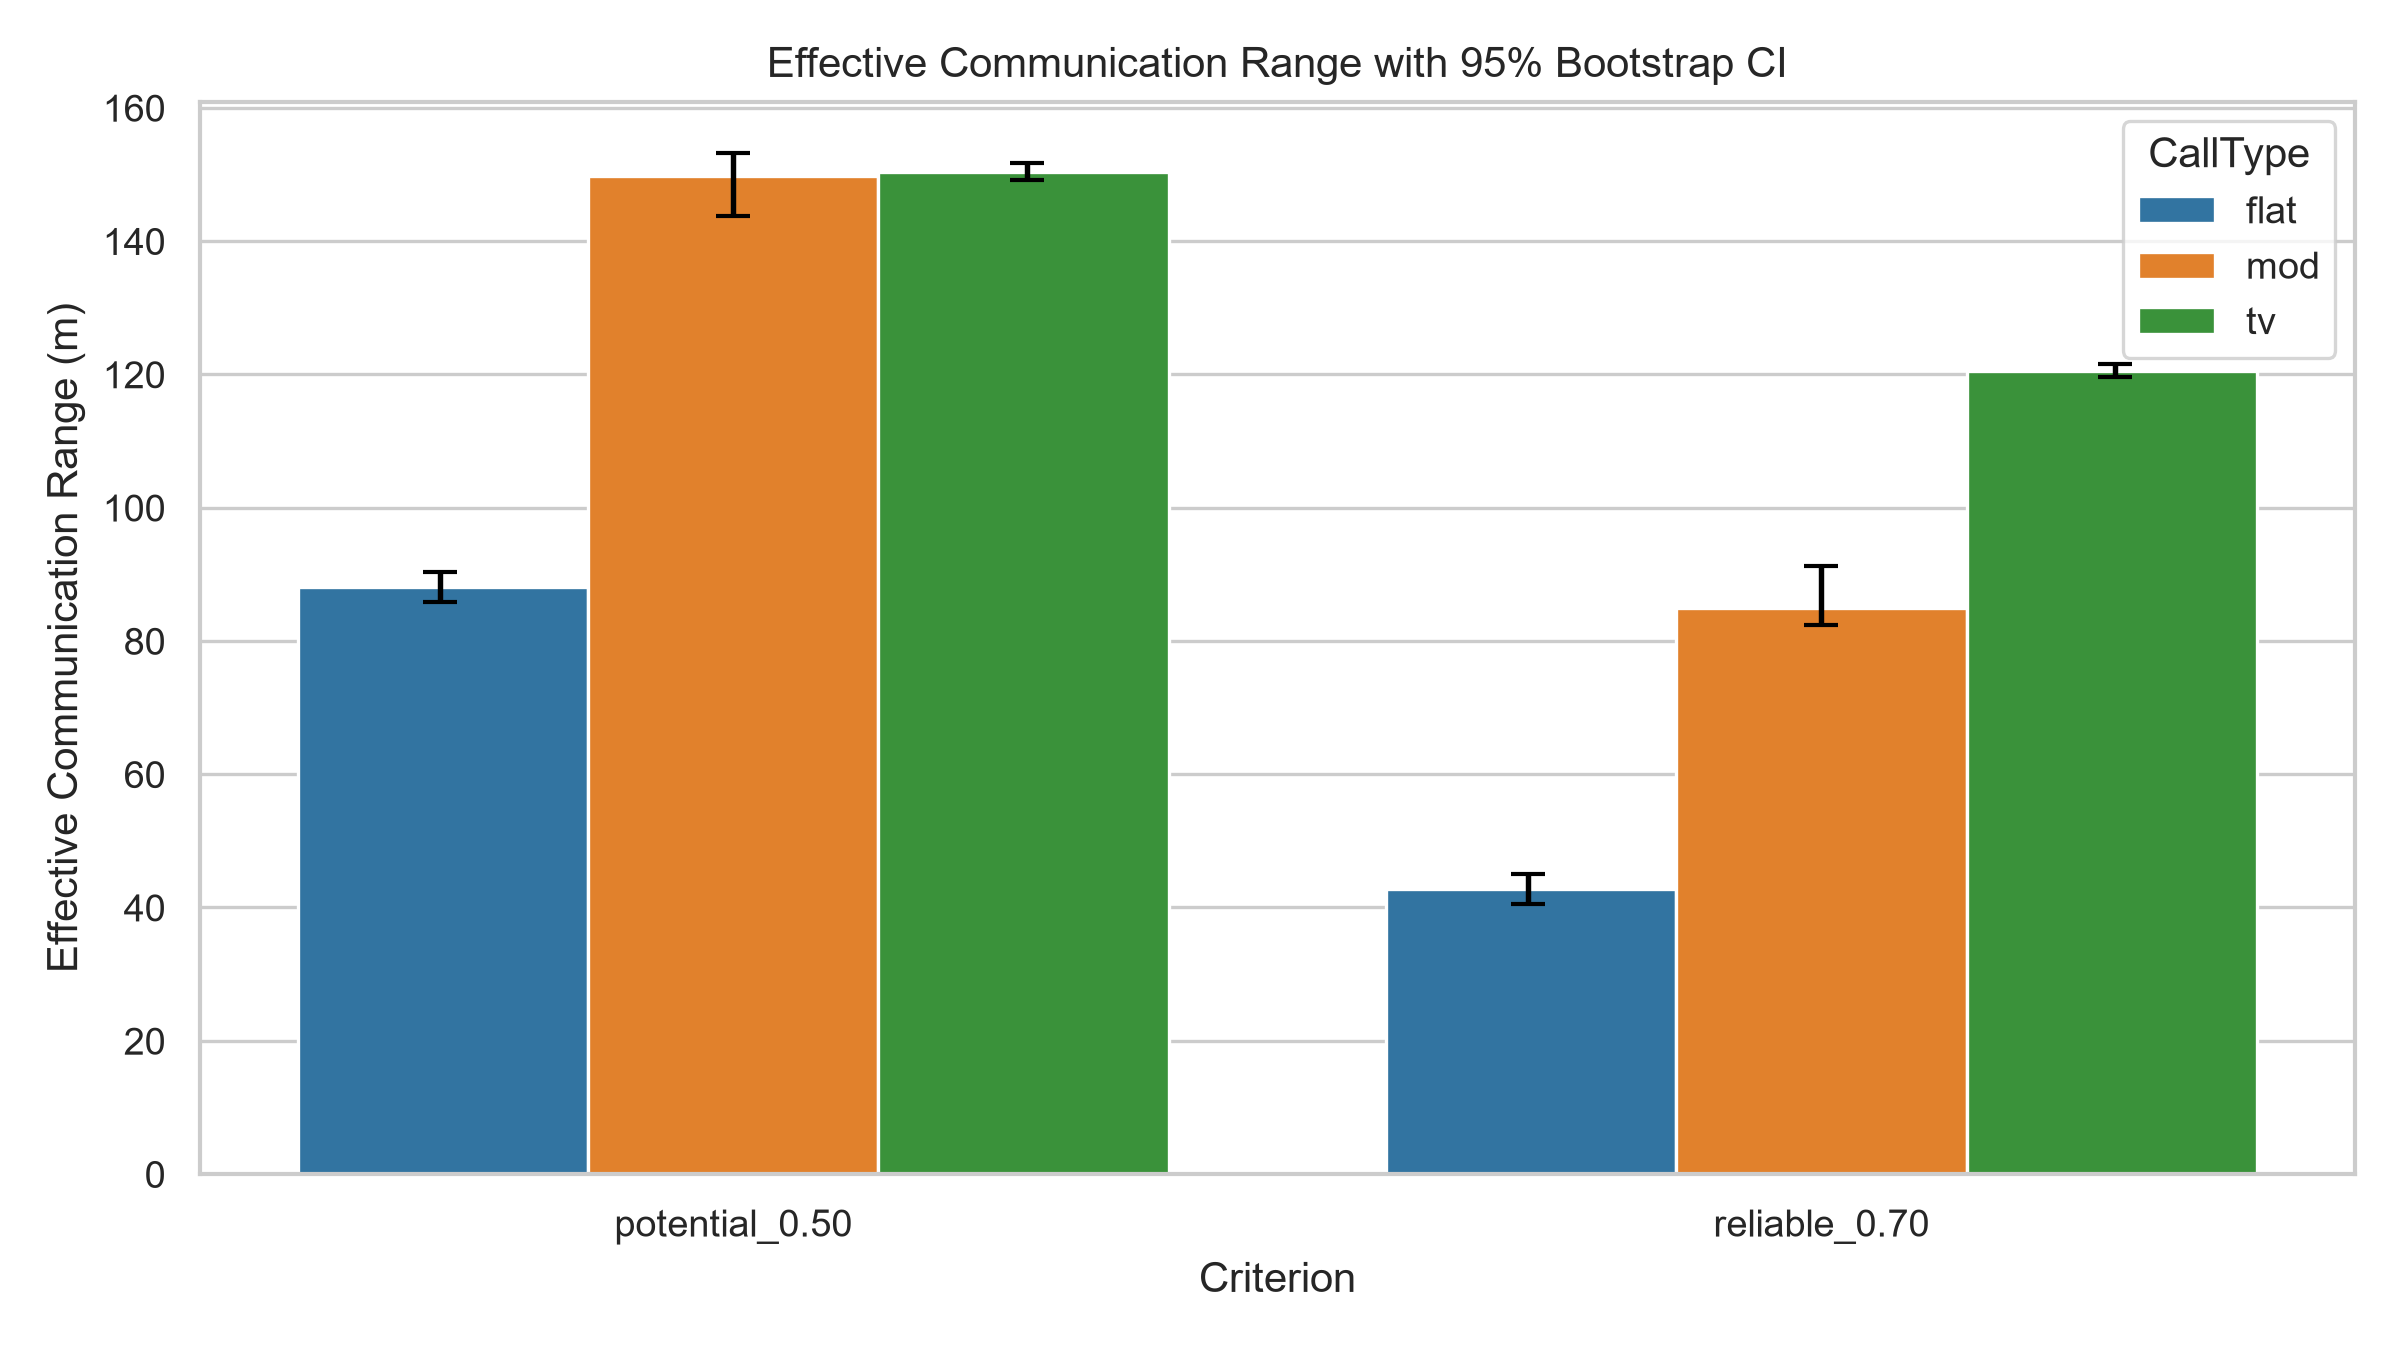
\includegraphics[width=0.95\textwidth]{q2_effective_range_ci.png}
\caption{Effective ranges at the potential (0.50) and reliable (0.70) thresholds with 95\%
bootstrap intervals.}
\label{fig:q2range}
\end{figure}

\subsection{Conclusion}
Two-voice calls preserve spectral and temporal structure to roughly 1.7 times the range of flat
calls at the potential-recognition criterion, and to roughly 2.8 times at the reliable
criterion. Modulated calls are intermediate but close to tv at the most permissive threshold.
This ranking is consistent with the structural difference identified in Problem 1: the second
voice band provides redundancy that survives propagation, whereas flat calls carry little
structure to lose.

% =====================================================================
\section{Problem 3: behavioural responses in playback experiments}

\subsection{Overall response rates and paired comparison}
Natural calls elicited a response in 90 of 139 trials (64.7\%) and control sounds in 18 of 139
(12.9\%; $\chi^2$ $p=2.4\times10^{-18}$). Because the two trials of an experiment are paired,
we also used an exact McNemar test: 74 pairs were discordant in favour of the call, 2 in favour
of the control, and 16 concordant ($p=7.7\times10^{-20}$). The result is unchanged when
restricted to the 49 pairs played at exactly the same distance ($p=1.6\times10^{-6}$), which
addresses the fact that call and control distances differ in 90 of 139 experiments.

\subsection{Response model}
We fitted a generalised estimating equation logistic model clustered by experiment,
\begin{equation}
\operatorname{logit}\,\Pr(Y_j=1)=\beta_0+\beta_k\,\mathrm{CallType}_j
+\beta_c\,\mathrm{Context}_j+\beta_d\log_2 d_j+\beta_n\log N_j ,
\end{equation}
with control as the reference category (Table~\ref{tab:gee}). All three call types raise the
odds of a response substantially: 14.0 (flat), 16.2 (mod) and 20.9 (tv) relative to control.
Each doubling of distance multiplies the odds by 0.63 (95\% CI 0.42--0.94, $p=0.022$), and
each e-fold increase in group size multiplies them by 0.60 (0.40--0.89, $p=0.012$). Context
effects are not significant after adjustment (commuting OR 0.89, searching OR 1.69), which
reflects confounding with call type: searching trials were more often assigned to tv calls.

\begin{table}[htbp]
\centering
\caption{GEE logistic model for the probability of any response (control = reference).}
\label{tab:gee}
\small
\begin{tabular}{lccl}
\toprule
Term & Odds ratio & 95\% CI & $p$ \\
\midrule
flat vs.\ control & 13.96 & 6.60--29.52 & $<0.001$ \\
mod vs.\ control & 16.16 & 6.42--40.70 & $<0.001$ \\
tv vs.\ control & 20.86 & 8.82--49.32 & $<0.001$ \\
Context: commuting & 0.89 & 0.36--2.18 & 0.791 \\
Context: searching & 1.69 & 0.59--4.88 & 0.329 \\
$\log_2$ distance (per doubling) & 0.63 & 0.42--0.94 & 0.022 \\
$\log$ group size (per e-fold) & 0.60 & 0.40--0.89 & 0.012 \\
\bottomrule
\end{tabular}
\end{table}

The negative group-size coefficient is counter-intuitive and should not be read causally.
Larger groups occurred mainly in the commuting context, where baseline responsiveness is lowest;
the coefficient therefore describes an association net of context and call type, not a
behavioural law.

\subsection{Response combinations}
Eight combinations of head-raising (H), vocalisation (V) and approach (A) were observed
(Table~\ref{tab:8state}). Control trials are dominated by ``none'' (87.1\%); natural calls
produce a broad distribution in which ``none'' falls to 35.3\%, with H+V (20.1\%), V alone
(20.9\%) and H+V+A (10.1\%) as the main alternatives. A chi-square test is unreliable here
because the minimum expected count is 0.50; a 5000-permutation test gives $p=0.0002$.

\begin{table}[htbp]
\centering
\caption{Probability of each response combination, control versus natural calls.}
\label{tab:8state}
\small
\begin{tabular}{lcc}
\toprule
Combination & Control & Natural calls \\
\midrule
None & 0.871 & 0.353 \\
Head-up only & 0.094 & 0.072 \\
Vocal only & 0.036 & 0.209 \\
Approach only & 0.000 & 0.007 \\
Head-up + vocal & 0.000 & 0.201 \\
Head-up + approach & 0.000 & 0.022 \\
Vocal + approach & 0.000 & 0.036 \\
All three & 0.000 & 0.101 \\
\bottomrule
\end{tabular}
\end{table}

\begin{figure}[htbp]
\centering
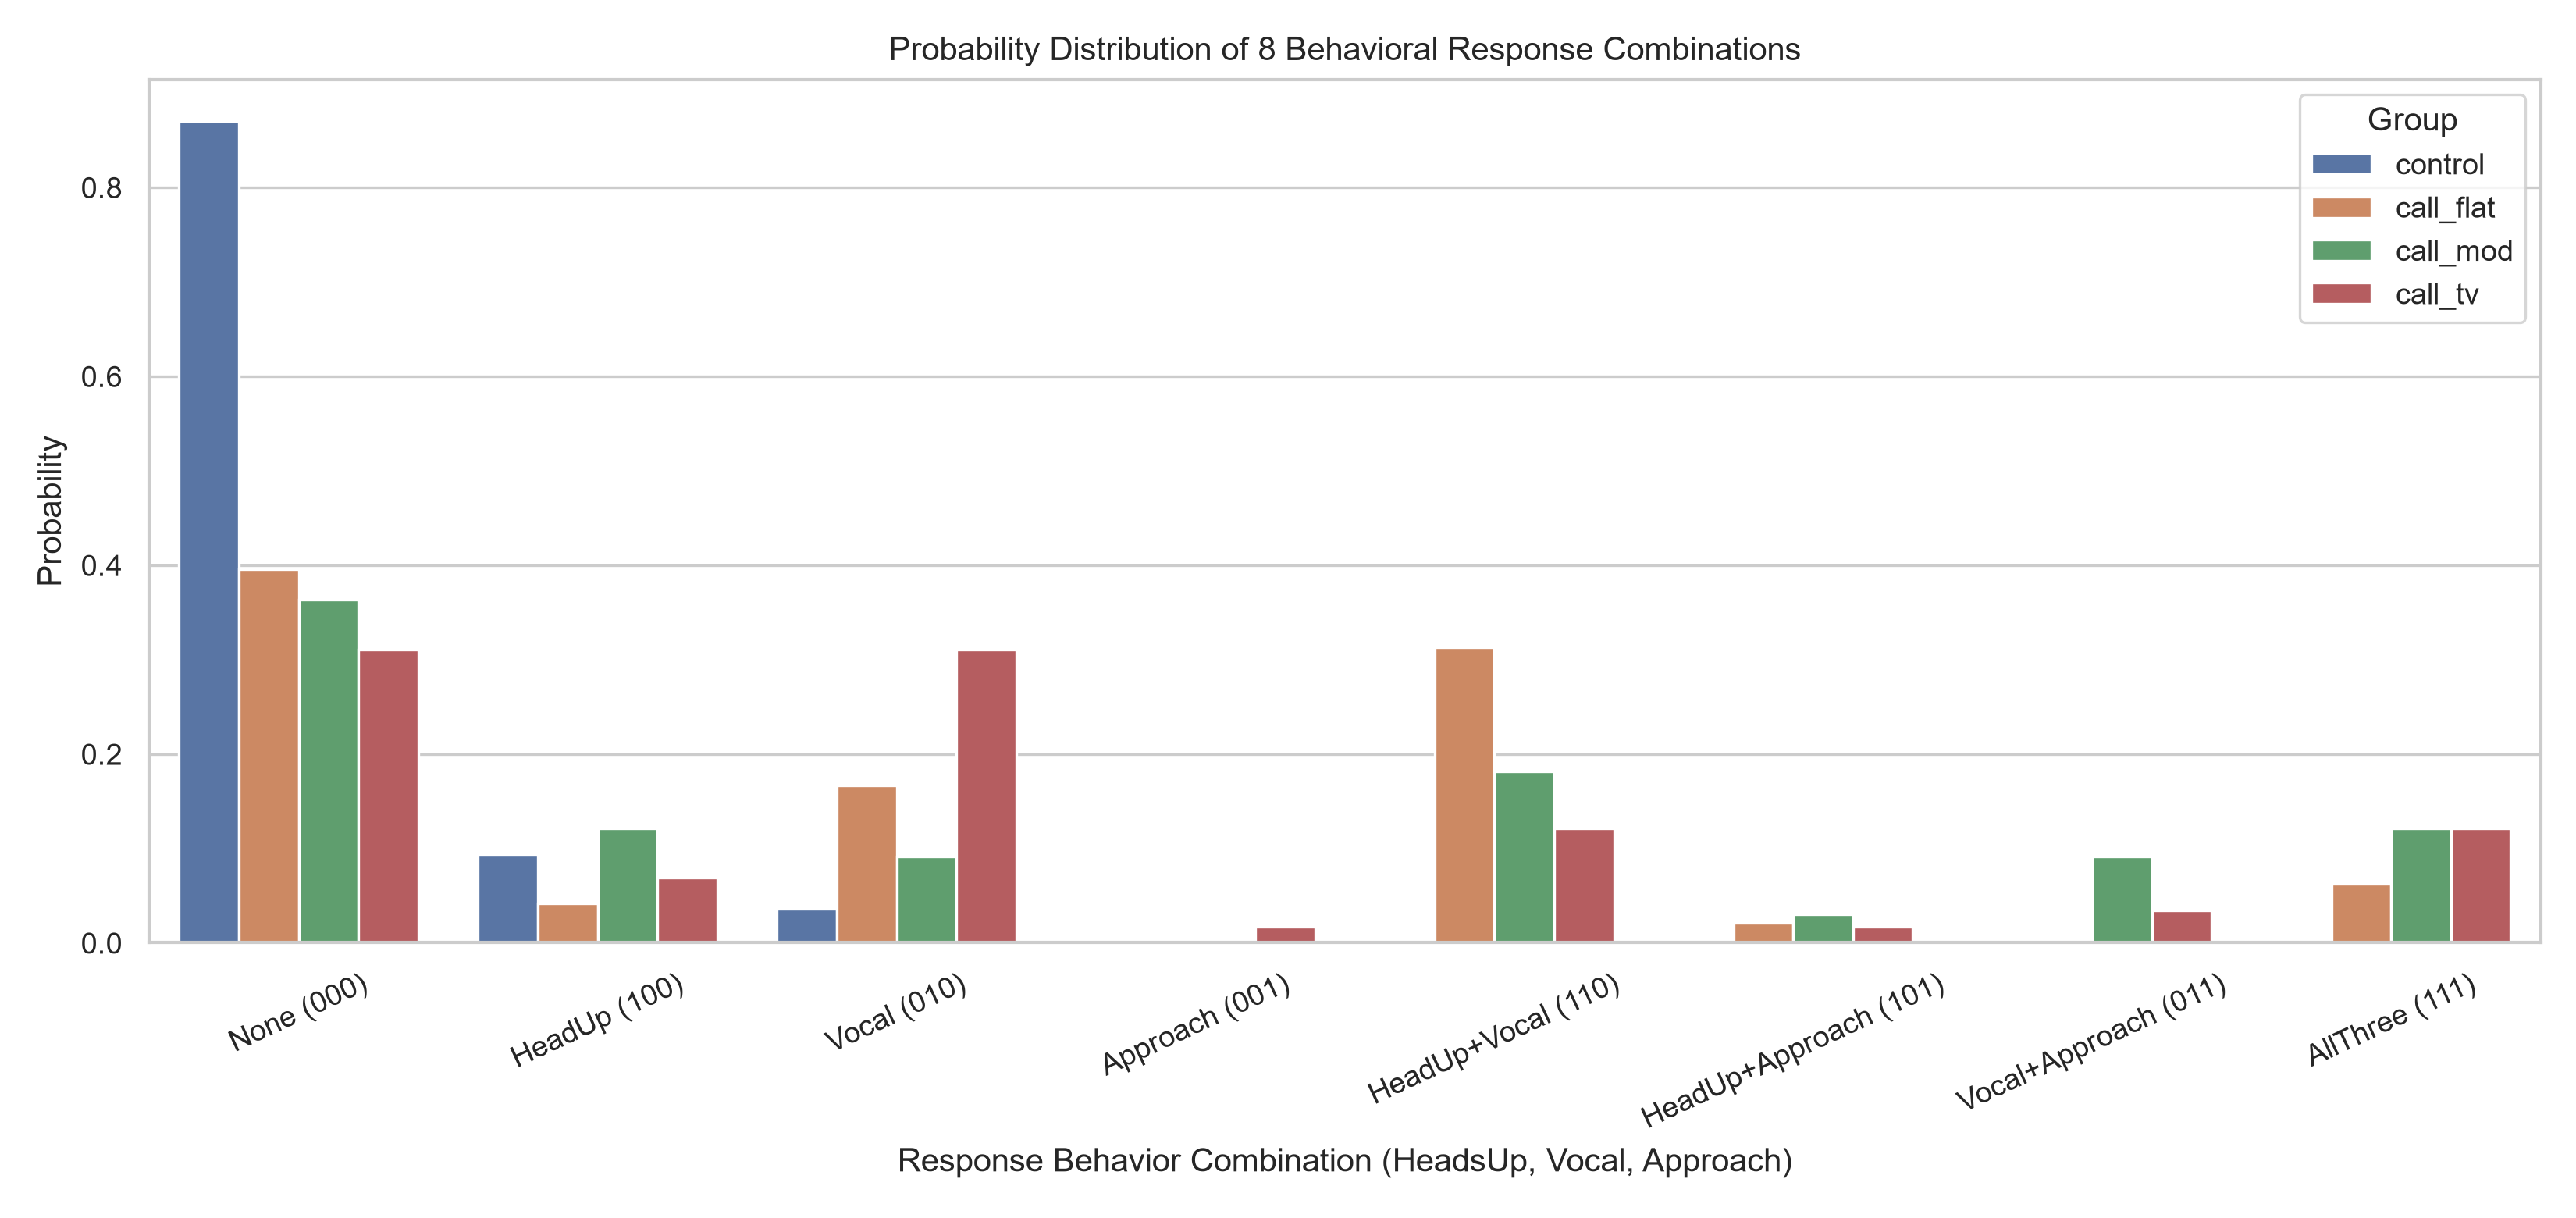
\includegraphics[width=0.95\textwidth]{q3_response_combinations.png}
\caption{Distribution of the eight behavioural response combinations.}
\label{fig:q3comb}
\end{figure}

\subsection{Latency model}
We use a hurdle structure. The first part is the GEE above, which gives the probability that a
response occurs at all. The second part is a log-normal model for latency \emph{among
responders}, fitted by least squares on $\log(\text{latency})$ with the same covariates. This
follows the problem's instruction that ``no response'' should be treated as no response rather
than as a very long latency. Table~\ref{tab:latency} reports predicted probabilities and median
initiation latency conditional on responding, at the median group size of eight and in the
searching context.

\begin{table}[htbp]
\centering
\caption{Predicted response probability and median initiation latency given a response
($N=8$, searching context).}
\label{tab:latency}
\small
\begin{tabular}{lcccccc}
\toprule
& \multicolumn{3}{c}{Response probability} & \multicolumn{3}{c}{Median initiation latency (s)} \\
\cmidrule(lr){2-4}\cmidrule(lr){5-7}
Call type & 50 m & 100 m & 150 m & 50 m & 100 m & 150 m \\
\midrule
flat & 0.742 & 0.644 & 0.580 & 1.71 & 2.00 & 2.19 \\
mod & 0.769 & 0.677 & 0.615 & 1.61 & 1.88 & 2.06 \\
tv & 0.811 & 0.730 & 0.674 & 2.35 & 2.75 & 3.01 \\
control & 0.170 & 0.115 & 0.090 & 1.76 & 2.06 & 2.25 \\
\bottomrule
\end{tabular}
\end{table}

The predicted latencies are consistent with the data: the observed median initiation latency is
2.05 s, and the predicted values span 1.6--3.0 s. Model calibration by distance bin is good at
short range (observed 0.488 vs.\ predicted 0.503 below 50 m; 0.331 vs.\ 0.351 at 50--100 m) and
acceptable at longer range, where the sample is small (0.421 vs.\ 0.332 at 100--150 m, $n=19$;
0.412 vs.\ 0.250 above 150 m, $n=17$).

\begin{figure}[htbp]
\centering
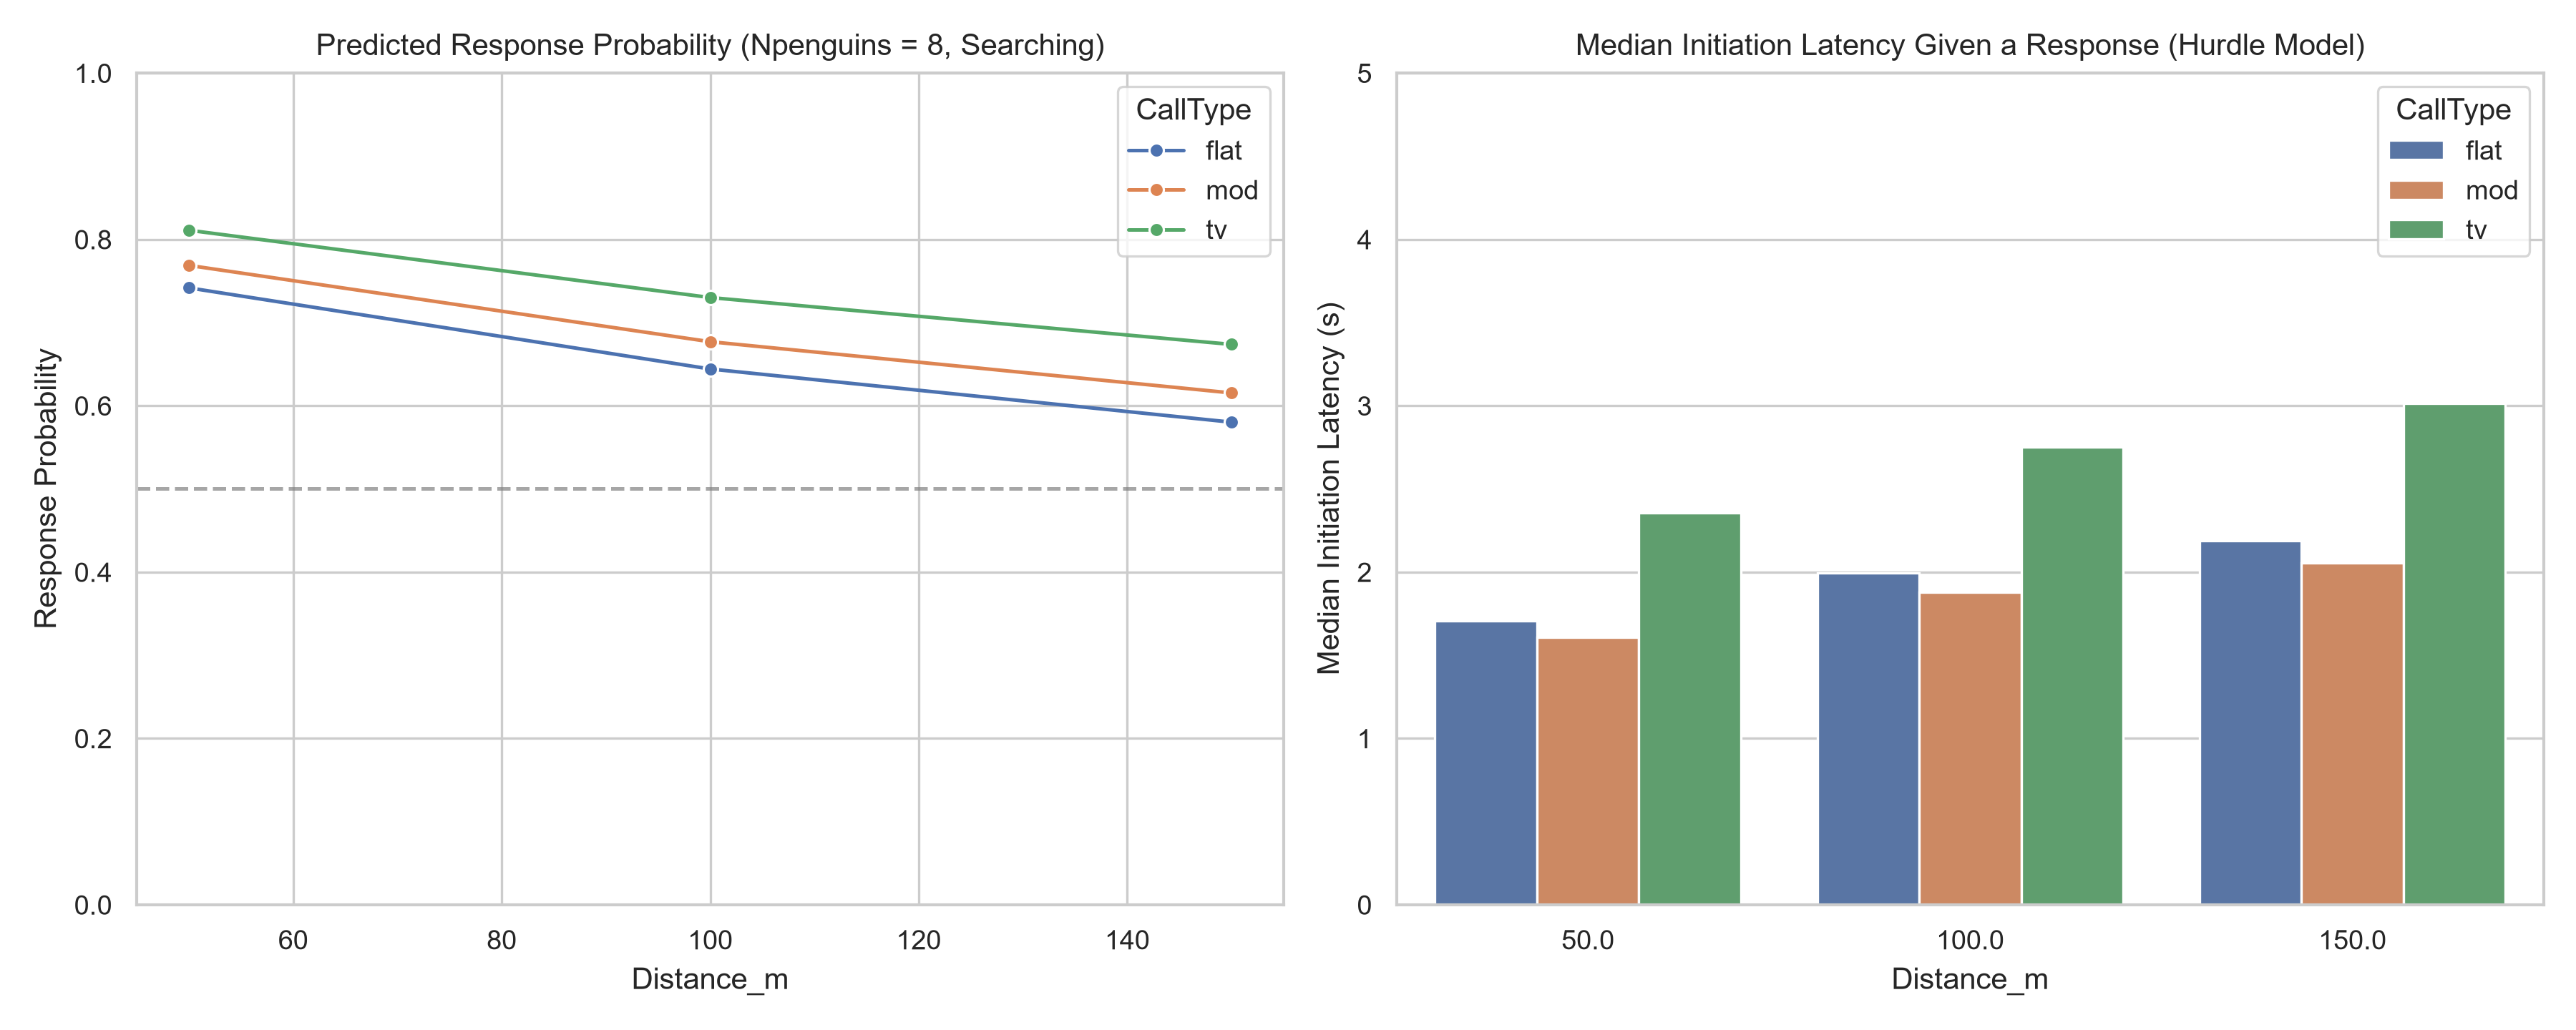
\includegraphics[width=0.95\textwidth]{q3_latency_predictions.png}
\caption{Predicted response probability and median initiation latency given a response.}
\label{fig:q3lat}
\end{figure}

\subsection{Sensitivity: censored AFT}
As a sensitivity analysis we also fitted a right-censored log-normal accelerated failure time
model in which non-responders are censored at 60 s. That model produces median head-up and
approach latencies beyond the observation window (and does not converge for approach, where
92\% of trials are censored). We report these as ``not estimable ($>60$ s)'' rather than as
numbers. The comparison supports the hurdle specification: treating non-response as censoring
forces a heavy tail that the data cannot identify, whereas the hurdle model yields stable,
interpretable medians.

\subsection{Response intensity}
The same hurdle logic is applied to the three intensity measures. Part 1 is a GEE model for the
probability that the behaviour occurs; part 2 models the positive values, using a
negative-binomial count model for vocalisation and censored log-normal models for durations
(values at the 60 s cap are censored). Approach duration has only 23 positive trials, 7 of them
censored, so its part-2 model is restricted to call type.

Among birds that vocalise, mod calls produce the most calls (5.8 versus 3.7 for flat and 3.8
for tv at 100 m), but the contrast is not significant ($p=0.119$); distance and group size do
not affect call counts. Head-up bouts are longer after mod ($+0.66$ on the log scale,
$p=0.002$) and tv ($+0.48$, $p=0.021$) than after flat, and shorter in larger groups
($-0.31$ per e-fold, $p=0.001$). Approach bouts are longest after tv (median 49 s versus 24 s
for flat), although with 23 events the call-type contrasts are not significant.

\begin{table}[htbp]
\centering
\caption{Response intensity at 100 m (group size 8, searching context).}
\label{tab:intensity}
\small
\begin{tabular}{lccc}
\toprule
 & flat & mod & tv \\
\midrule
\multicolumn{4}{l}{\emph{Vocalisation}} \\
P(vocalise) & 0.66 & 0.60 & 0.72 \\
Calls per trial ($P\times$ mean) & 2.44 & 3.45 & 2.76 \\
\midrule
\multicolumn{4}{l}{\emph{Head-up}} \\
P(head-up) & 0.34 & 0.35 & 0.25 \\
Median duration (s) & 14.9 & 23.6 & 19.8 \\
Expected seconds per trial & 5.1 & 8.2 & 4.9 \\
\midrule
\multicolumn{4}{l}{\emph{Approach}} \\
P(approach) & 0.06 & 0.19 & 0.16 \\
Median duration (s) & 23.7 & 34.7 & 49.3 \\
Expected seconds per trial & 1.5 & 6.6 & 7.9 \\
\bottomrule
\end{tabular}
\end{table}

Expected values are the product of the behaviour probability and the conditional central value.
For counts the central value is the model mean; for durations it is the median, because under
censoring the conditional mean is pulled towards the 60 s ceiling (56.7 s for tv approach).

Three patterns are worth noting. First, the intensity ranking differs from the probability
ranking: mod, not tv, produces the most vocalisations and the longest head-up bouts, whereas tv
produces the longest approach bouts. This is consistent with a division of function in which
modulated calls sustain contact once a response has begun, while two-voice calls are more likely
to recruit movement. Second, the negative group-size coefficient for head-up duration mirrors
the negative coefficient in the response model and should not be read causally. Third, the
approach model is the least certain: with 23 positive trials and 30\% of them censored at 60 s,
only the call-type contrast is retained, and none of the contrasts reaches significance.

% =====================================================================
\section{Problem 4: communication effectiveness and conservation scenarios}

\subsection{Index definition}
We define the effectiveness index as the geometric mean of signal fidelity and behavioural
utility,
\begin{equation}
E_k(c,d)=\sqrt{F_k(d)\;U_k(c,d)},\qquad
U_k(c,d)=P_k(c,d)\sum_{r=1}^{4}\frac{\pi_{k,r}(c,d)}{1-\pi_{k,0}(c,d)}\,u_r ,
\end{equation}
where $P_k(c,d)$ is the response probability from the Problem-3 GEE model, $\pi_{k,r}$ is the
predicted probability of response tier $r$ from the multinomial model, and $u_r$ is an
ecological utility assigned to each tier: none 0, head-up only 0.25 (vigilance), vocal only
0.50 (acoustic contact), head-up + vocal 0.75 (attentive reply), approach involved 1.00
(cohesion and recruitment).

The GEE supplies the overall probability that any response occurs; the multinomial model
supplies only the composition across tiers conditional on responding, renormalised by
$1-\pi_{k,0}$. The index therefore uses the same probability model as Section 8.2 rather than a
second, competing one. The two models agree closely on the 147 grid points: the mean absolute
difference in response probability is 0.046, with a maximum of 0.137.

The geometric mean expresses the fact that communication requires both a detectable signal and
a behaviourally meaningful response: a perfect signal with no response, or a strong response to
an unrecognisable signal, should not score highly.

The index is a \emph{relative} scale, not a probability. At 10 m it reaches about 0.70 rather
than 1.0, because 11--16\% of trials produce no response even at close range and because the
utility ceiling is 1.0.

\subsection{Effectiveness profiles}
At a typical group size of eight and averaging over the observed context mix, the index declines
from about 0.70 at 10 m to 0.21--0.28 at 250 m (Table~\ref{tab:q4index}). Tv and mod are similar
at short range, but tv separates from mod beyond 100 m; flat is consistently lowest.

\begin{table}[htbp]
\centering
\caption{Communication effectiveness index by distance (group size 8, context-weighted).}
\label{tab:q4index}
\small
\begin{tabular}{lccccc}
\toprule
Call type & 10 m & 50 m & 100 m & 150 m & 250 m \\
\midrule
flat & 0.703 & 0.544 & 0.401 & 0.309 & 0.208 \\
mod & 0.701 & 0.609 & 0.508 & 0.412 & 0.268 \\
tv & 0.697 & 0.605 & 0.542 & 0.414 & 0.281 \\
\bottomrule
\end{tabular}
\end{table}

\begin{figure}[htbp]
\centering
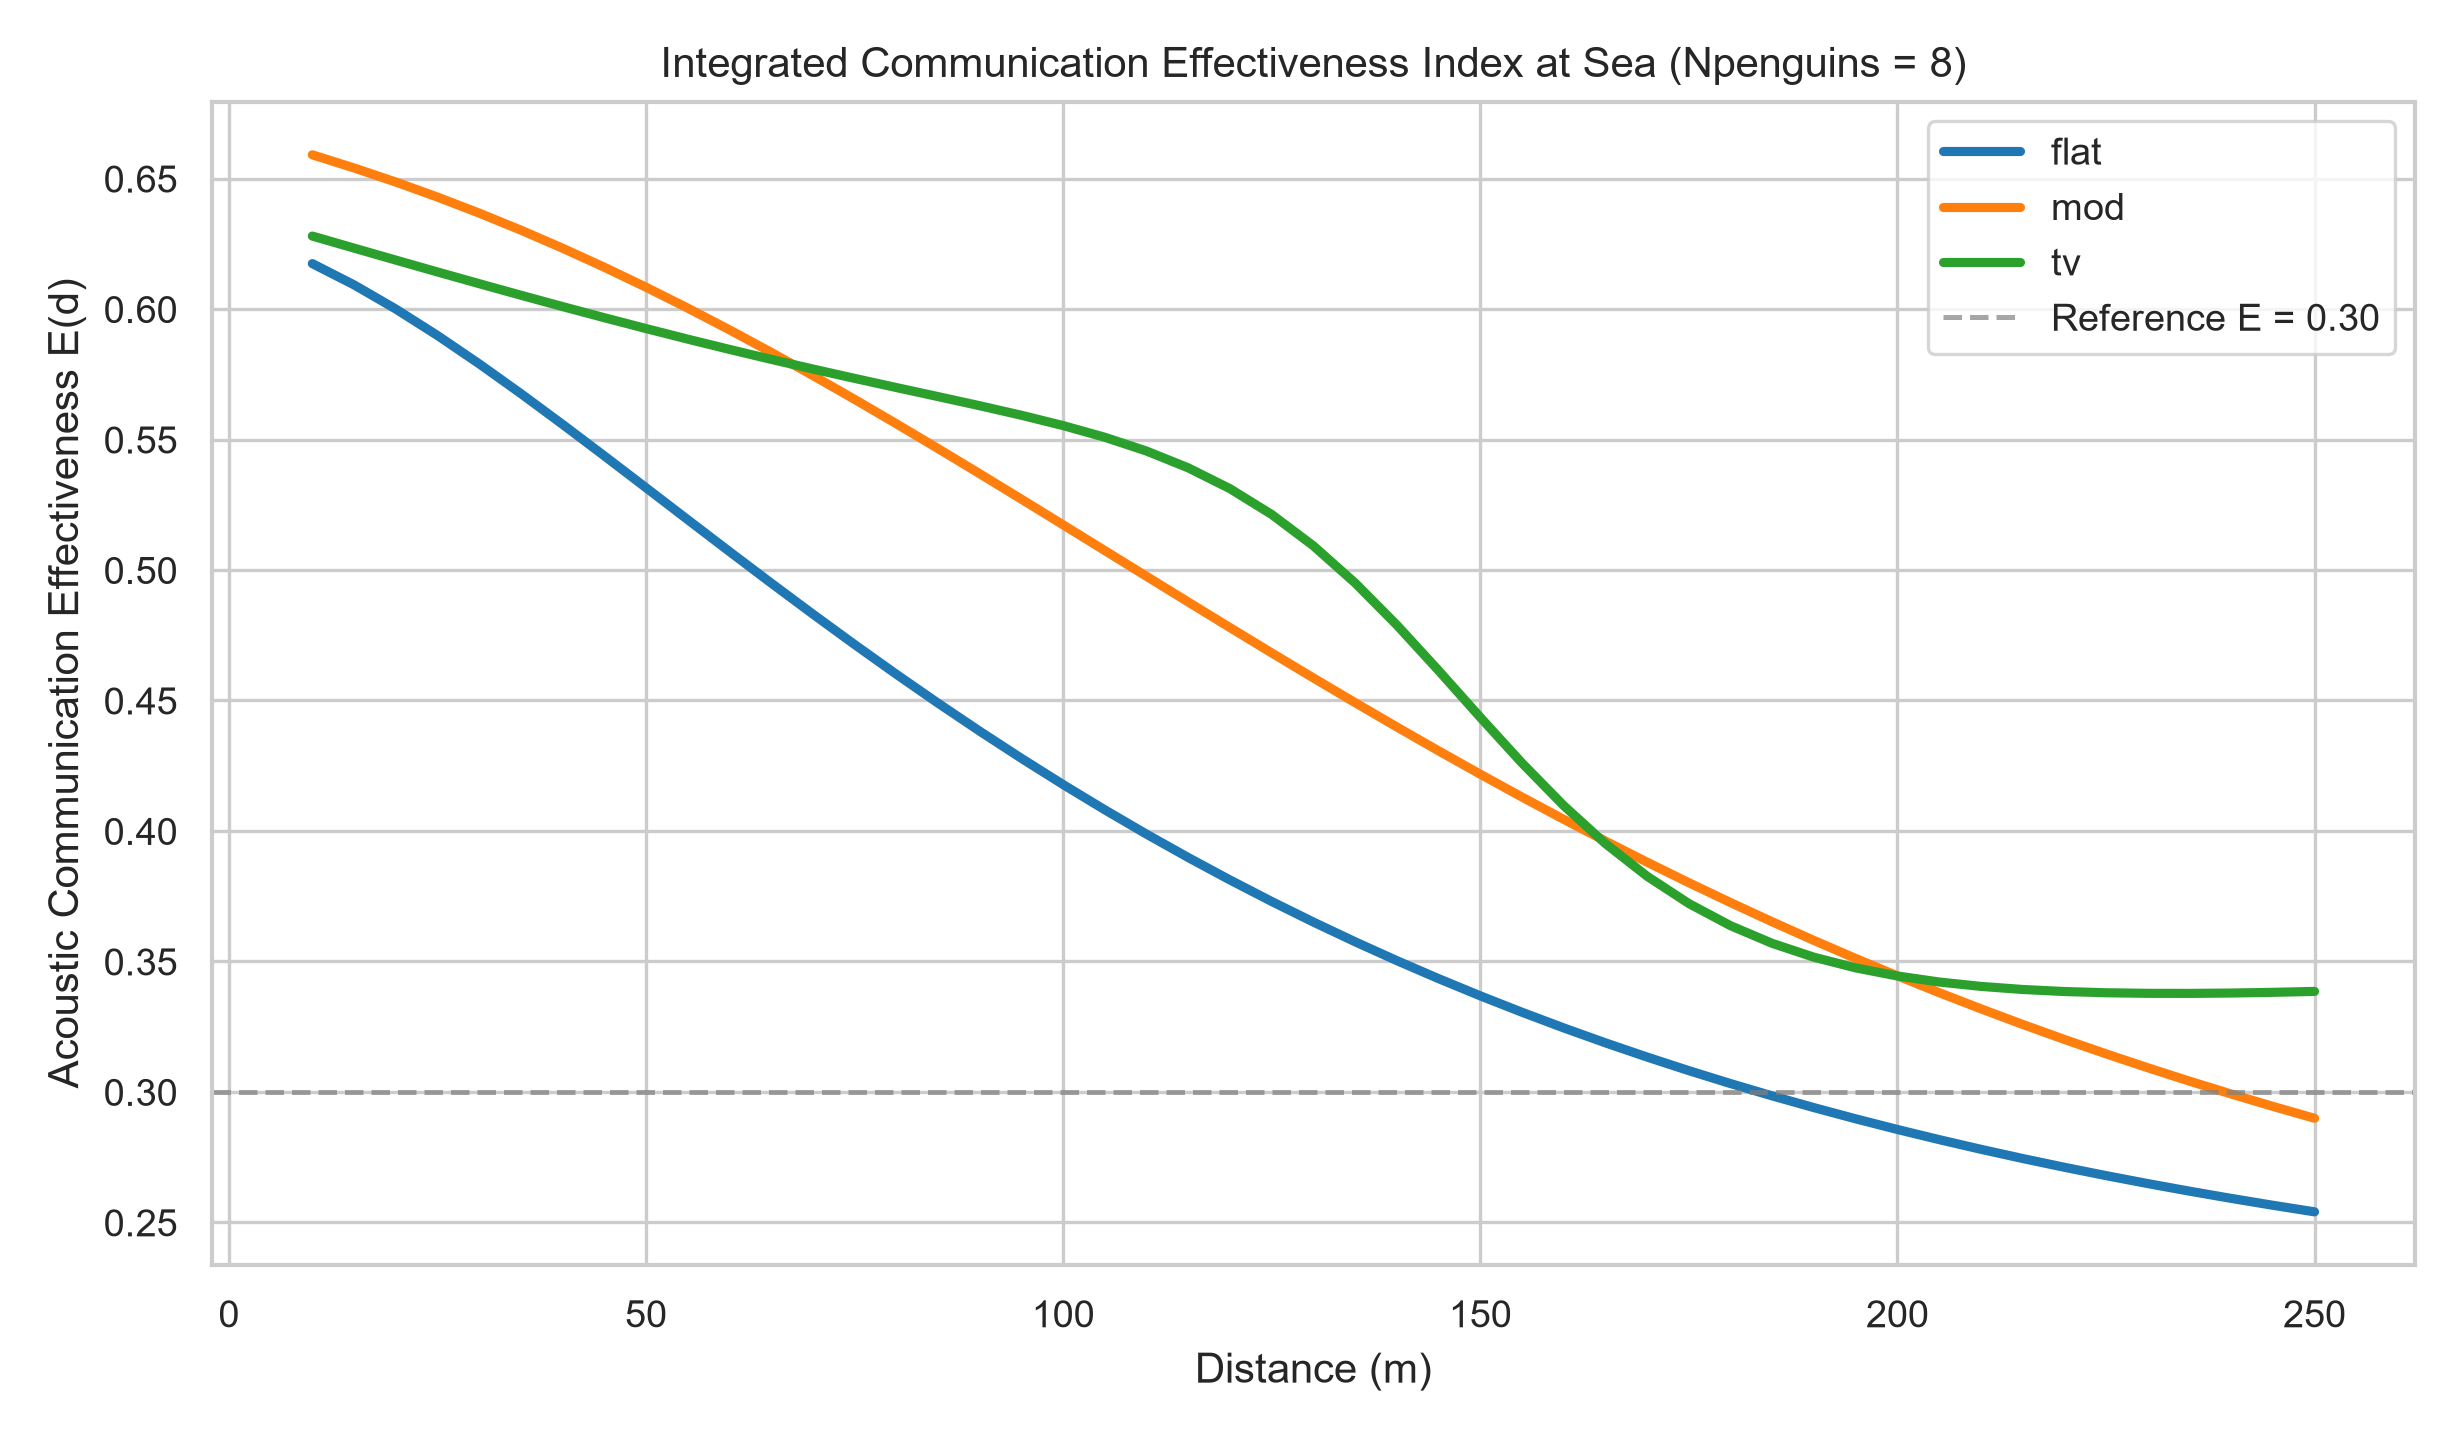
\includegraphics[width=0.9\textwidth]{q4_effectiveness_curves.png}
\caption{Communication effectiveness index versus distance.}
\label{fig:q4eff}
\end{figure}

\subsection{Expected responders}
To translate the group-level response probability into an expected count, we assume
homogeneous individuals, convert the predicted group probability $p^{\text{trial}}$ into an
individual probability $p^{\text{ind}}=1-(1-p^{\text{trial}})^{1/N}$, and scale by the assumed
proportion $\rho$ of responsive individuals:
$\mathbb{E}[n_{\text{resp}}]=N\rho\,p^{\text{ind}}$.
At $N=8$ and $\rho=0.5$, the expected counts at 50/100/150 m are 0.62/0.48/0.41 for flat,
0.67/0.53/0.45 for mod and 0.75/0.60/0.52 for tv. These are deliberately conservative: a
group-level response of 70\% does not imply that 70\% of individuals respond.

\subsection{Scenarios}
Raising the recognition threshold from 0.50 to 0.60 and 0.70 shortens the radius of flat calls
from 88 m to 64 m and 43 m, that of mod from 150 m to 118 m and 85 m, and that of tv from 150 m
to 138 m and 121 m (Table~\ref{tab:q4scen}). A 20\% reduction in signal correlation at all
distances has a much stronger effect on flat (88 to 59 m, relative reading) than on tv (150 to
134 m). Under the absolute reading of the same scenario (correlation reduced by 0.20), the
radii become 43/85/121 m, identical to the 0.70-threshold case because the two manipulations
coincide at that point.

\begin{table}[htbp]
\centering
\caption{Effective radius (m) under noise scenarios.}
\label{tab:q4scen}
\small
\begin{tabular}{lcccc}
\toprule
Call type & Baseline & $\theta=0.60$ & $\theta=0.70$ & Corr.\ $-20\%$ (rel./abs.) \\
\midrule
flat & 88.0 & 64.4 & 42.7 & 59.0 / 42.7 \\
mod & 149.7 & 118.0 & 85.0 & 110.1 / 85.0 \\
tv & 150.4 & 137.7 & 120.5 & 134.3 / 120.5 \\
\bottomrule
\end{tabular}
\end{table}

\begin{figure}[htbp]
\centering
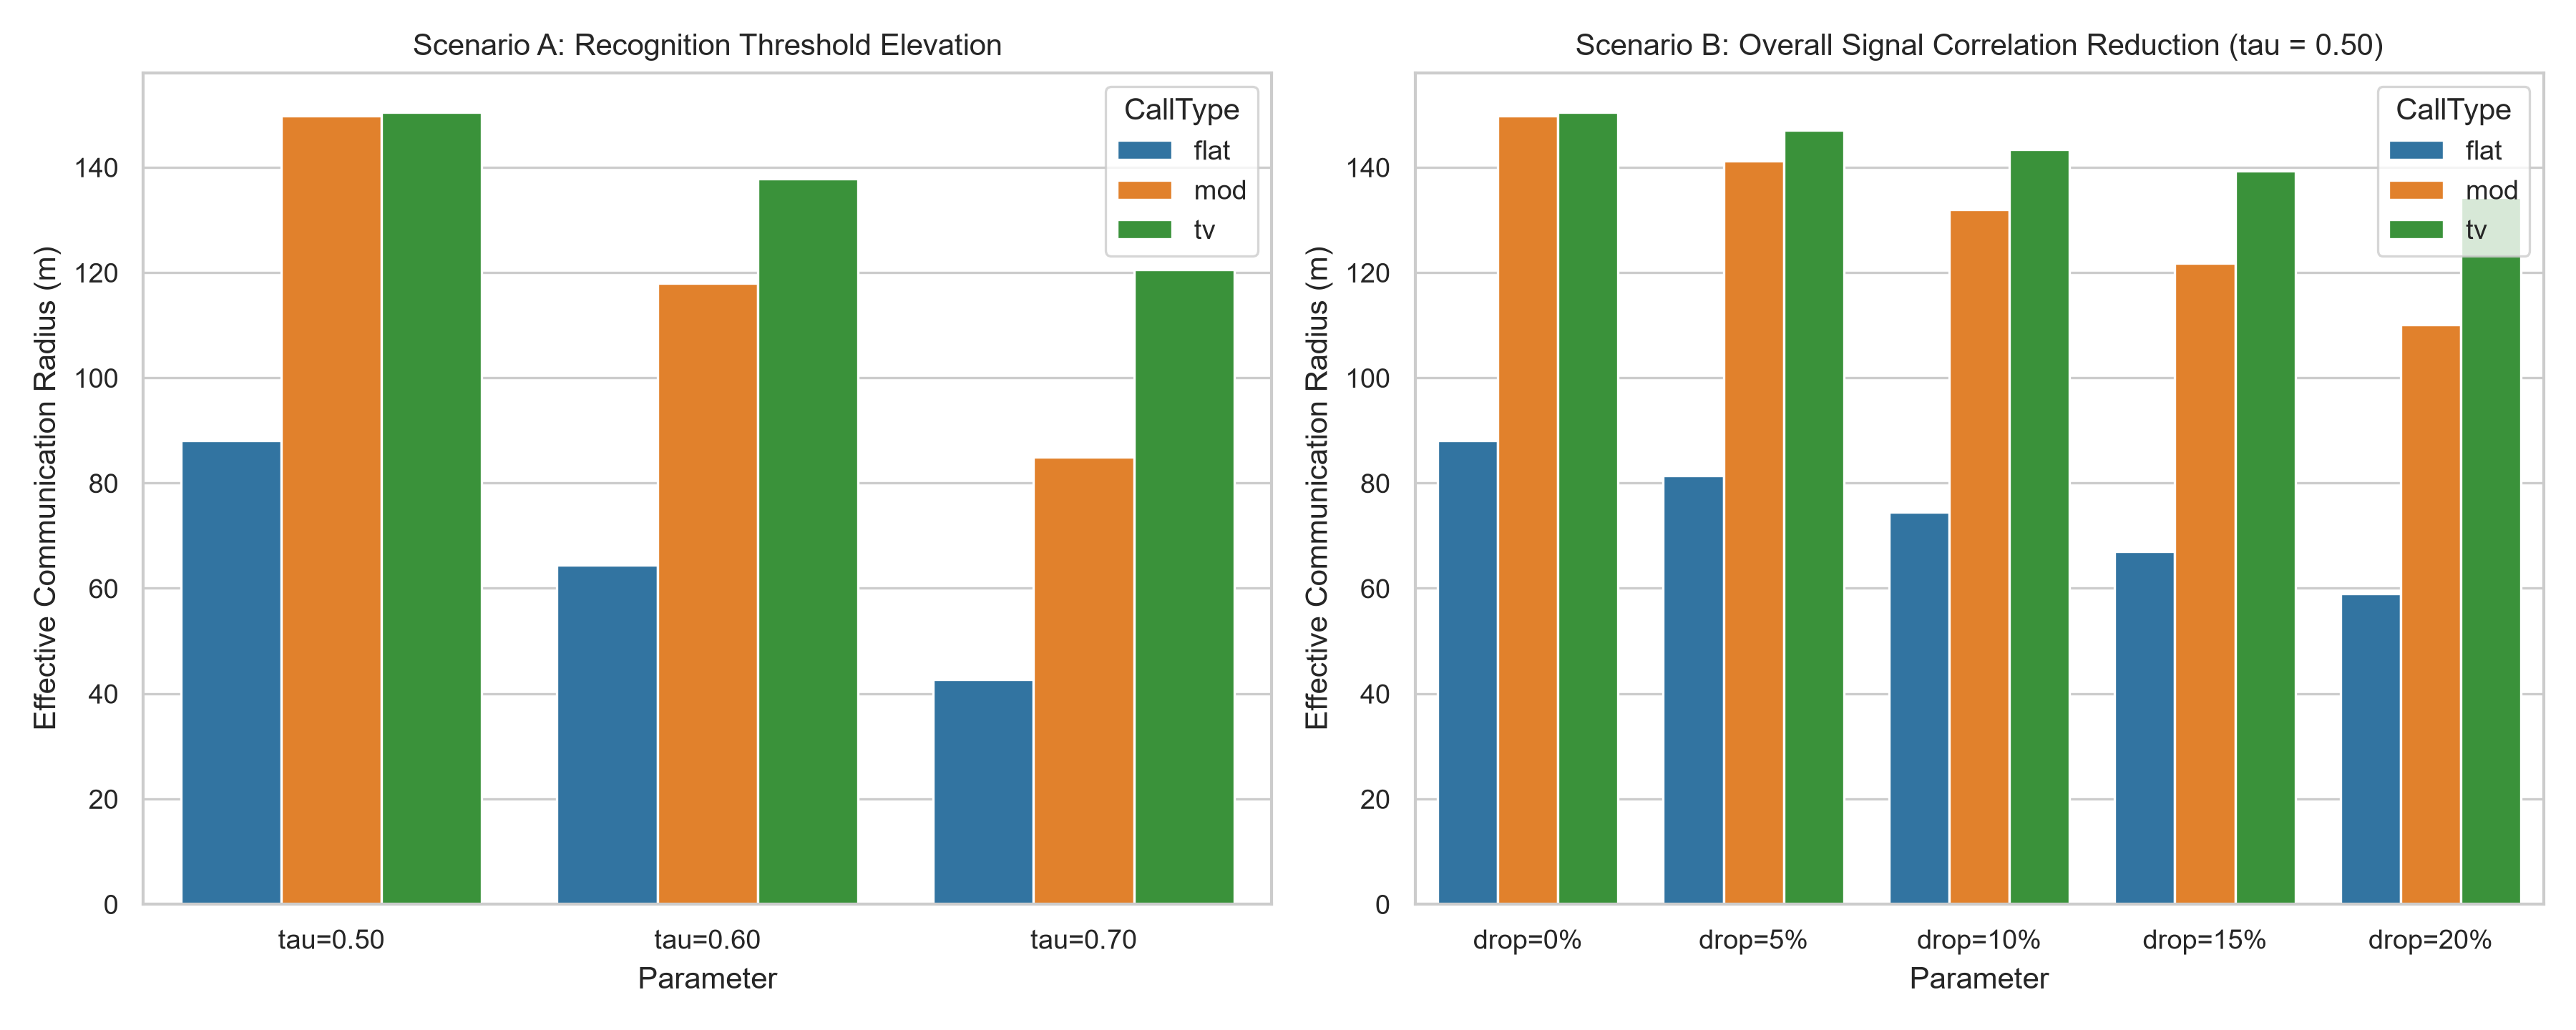
\includegraphics[width=0.95\textwidth]{q4_noise_scenarios.png}
\caption{Effective radius under threshold elevation and signal-correlation reduction.}
\label{fig:q4scen}
\end{figure}

Two results deserve comment. First, the response probability \emph{at the effective radius}
increases slightly as the threshold becomes stricter (for example 0.66 to 0.76 for flat). This
is not paradoxical: a stricter criterion places the radius closer to the source, where responses
are more likely. Second, the expected number of responders therefore changes little across
scenarios even though the radius shrinks substantially; the two quantities answer different
questions and should be reported separately.

\subsection{Conservation implications}
The results support three conditional recommendations.

\textbf{(i) Protect a noise-limited core around foraging aggregations.} Because tv calls remain
recognisable to about 120 m under the most stringent threshold, a core zone of this order
represents the distance over which group cohesion can be maintained acoustically. The
recommendation applies to foraging areas used by groups of the observed size (median 8) and
assumes that call recognition, not visual contact, is the limiting channel.

\textbf{(ii) Regulate vessel activity rather than only vessel presence.} The scenario analysis
shows that a 10\% relative loss of signal correlation costs flat calls about 15\% of their radius
but tv calls less than 5\%. Management that reduces broadband noise during foraging hours
therefore protects the most vulnerable call type disproportionately.

\textbf{(iii) Prioritise areas where flat calls dominate.} If a colony or foraging ground relies
mainly on flat calls, the same noise increase removes a much larger fraction of the communication
range. Surveys of call-type use could therefore inform spatial prioritisation.

These recommendations are conditional. The data cover two locations in False Bay and a single
study period, the playback distances do not exceed 200 m, and the fidelity index is a relative
signal measure rather than a hearing threshold. The recommendations should be treated as
hypotheses for monitoring, not as fixed setback distances.

% =====================================================================
\section{Validation and sensitivity summary}

To verify robustness across all four problems, we evaluated out-of-sample generalisation, model calibration, residual diagnostics, and parameter sensitivity. Table~\ref{tab:validation} summarises the validation protocols and sensitivity checks across the full modelling pipeline.

\begin{table}[htbp]
\centering
\caption{Summary of model validation.}
\label{tab:validation}
\small
\begin{tabularx}{\textwidth}{@{}l>{\raggedright\arraybackslash}X>{\raggedright\arraybackslash}X>{\raggedright\arraybackslash}X@{}}
\toprule
Model & Diagnostic & Generalisation / calibration & Sensitivity \\
\midrule
Classifiers & Grouped CV; permutation test & Macro-F1 0.385, permutation $p=0.133$; structural key 0.944 & Single-voice subset 53.6\% vs.\ 52.4\% baseline \\
Fidelity curves & Residuals; 4PL best AIC & $R^2$ 0.968--0.994; leave-one-distance check & Six weighting schemes; threshold 0.45--0.80 \\
Response model & GEE clustered by experiment & Calibration gaps 0.015--0.162 & Matched-distance 49 pairs; McNemar \\
Latency and intensity & Hurdle; NB / censored log-normal & Predicted 1.6--3.0 s vs.\ observed 2.05 s & AFT censoring: non-estimable medians \\
Effectiveness index & Baseline at 10 m (0.68--0.71) & Consistent ranking with Problem 2 & Weight grid; relative vs.\ absolute noise \\
\bottomrule
\end{tabularx}
\end{table}

% =====================================================================
\section{Discussion and limitations}

The central empirical finding is negative and useful: scalar acoustic summaries do not separate
the three call types, whereas structural features do. This has a practical consequence for
monitoring. Automated call classification should be built on spectro-temporal representations
rather than on a handful of summary statistics, and the near-perfect structural key suggests
that a simple two-stage rule may outperform a complex classifier on small samples.

Several limitations must be stated. The sample is small (108 calls, 139 experiments) and
geographically concentrated. Call-level individual identity is unknown, so cross-validation was
grouped by date as a proxy; residual leakage cannot be excluded. The propagation data provide
relative correlations, not absolute sound pressure, so the effective ranges are statements about
signal similarity rather than about audibility. Environmental covariates (sea state, wind,
ambient noise) were not recorded; their effect is absorbed into residual variance and may bias
the distance coefficient. The 60 s observation window censors long behaviours, and the playback
distances (5--200 m) do not overlap fully with the propagation distances (4--256 m). Finally,
the effectiveness index requires weights and a responsive-individual proportion that the data
cannot estimate; these are value judgements, and we have reported their sensitivity rather than
presenting a single number as definitive.

% =====================================================================
\section{Conclusion}

We combined acoustic measurements, propagation experiments and playback trials to quantify how
far African penguin calls remain recognisable at sea and how strongly penguins respond. Three
conclusions follow. First, call types are defined by voice structure, not by scalar summaries:
a structural key classifies 94.4\% of calls, while scalar classifiers perform at chance. Second,
two-voice calls are the most robust long-range signal, retaining roughly 1.7 times the
potential-recognition range and 2.8 times the reliable-recognition range of flat calls, and this
ranking survives every weighting scheme and threshold tested. Third, natural calls raise the
group response probability from 13\% to 65\%, and the effect of distance is modest but
detectable (odds ratio 0.63 per doubling), with responses typically beginning within two to
three seconds. The integrated index shows that the advantage of two-voice calls grows with
distance and under noise, which supports spatially explicit, call-type-aware management of
foraging habitat.

% =====================================================================
\begin{thebibliography}{9}
\bibitem{kw} Kruskal, W. H., and Wallis, W. A. (1952). Use of ranks in one-criterion variance analysis. \textit{Journal of the American Statistical Association}, 47(260), 583--621.
\bibitem{holm} Holm, S. (1979). A simple sequentially rejective multiple test procedure. \textit{Scandinavian Journal of Statistics}, 6(2), 65--70.
\bibitem{gee} Liang, K.-Y., and Zeger, S. L. (1986). Longitudinal data analysis using generalized linear models. \textit{Biometrika}, 73(1), 13--22.
\bibitem{efron} Efron, B., and Tibshirani, R. J. (1993). \textit{An Introduction to the Bootstrap}. Chapman and Hall.
\bibitem{aic} Burnham, K. P., and Anderson, D. R. (2002). \textit{Model Selection and Multimodel Inference}. Springer.
\bibitem{iucn} IUCN (2024). \textit{Spheniscus demersus}. The IUCN Red List of Threatened Species.
\bibitem{data} Data and supplementary materials for the 2026 APMCM Problem C. \url{https://zenodo.org/records/21376649}.
\end{thebibliography}

\newpage
\appendix
\renewcommand{\thesection}{\Alph{section}}
\setcounter{section}{0}
% The class hard-codes \Roman{section} in the section title format, so the
% body heading must be overridden separately from the TOC entry.
\titleformat{\section}{\centering\normalfont\Large\bfseries}{\Alph{section}.}{.5em}{}
\section{Code and reproducibility}
All analyses are implemented in Python and organised as four scripts
(\path{q1_acoustics_classification.py}, \path{q2_signal_degradation.py},
\path{q3_playback_responses.py}, \path{q4_effectiveness_conservation.py}).
Running them in order regenerates every table and figure in this paper; the random seed is
fixed at 42. The eleven input files are described in the README.

\end{document}
